\chapter{实现细节}
\label{chap:implements}
前一章中,我们已经介绍了整个系统的架构设计,这一章我们会对系统各个模块的一些实现细节进行详细阐述,主要涉及到方案选取、环境部署、算法设计与实现、系统性能调优等。一方面是对整体架构设计的补充论述,另一方面,我们会更多的讨论在实现过程中遇到的各种问题,以及如何解决这些问题。整体上,我们会倾向去寻找已有的成熟解决方案,辅以适当的修改和优化。遵循这个原则,既保证了整个系统有一定的成熟度,又对病历数据的识别有较强的针对性。这一部分的阐述比较详细,按照这一章的指引,有一定计算机编程基础的读者,应该能实现整个系统的基本复现。

\section{核心方案}
医学档案的自动生成与归类,其涉及到的最核心的两项技术就是图像处理和文字识别,可以说这两项技术的解决方案选取和完成度,决定了整个系统的性能基线,因此,我们必须综合考量备选的各个方案,从性能、稳定性、易用性等维度,择优采用。接下来,我们就这两项技术的方案选取和部署来展开讨论。

\subsection{图像处理}
\subsubsection{方案选取}
图像处理(Image Processing),通常又称数字图像处理,它将输入的图片、图片组或者是视频经过一系列的信号处理方面的数学转换,得到处理后的图片或是与图片相关的参数产出\citep{gonzalez2008digital}。本质来说,图像处理技术是将图片当做一个二维的信号,然后将标准的信号处理技术应用其上,当然,当图像处理技术运用到视频中时,输入变成了三维的信号,这第三维就是时间。近些年来,随着计算机视觉的蓬勃发展,图像处理技术也受到越来越多的关注。

结合前一章的分析我们可以看到,整个系统的六个模块(\autoref{pic:system-framework})中,数据加载模块、版面分析模块、预处理模块都需要用到图像处理的技术,因此我们有必要综合所有模块的需求,选取一个合适的图像处理解决方案。目前比较主流的图像处理类库有OpenCV\citep{bradski2008OpenCV}、EmguCV\citep{Shi013emgu}、AForge.net\citep{Kirillov2013Aforge}、CImg\citep{tschumperle2012cimg}等,在\citep{XianrongWang}的文章中,作者对几大主流的的图像处理库在各个维度做了一个比较全面的对比。从\autoref{pic:image-processing-comparison}中可以看到,OpenCV在性能上,是其中的佼佼者,也是最为广泛使用的图像处理类库,在功能上,也能完全满足本系统的图像处理要求,故经过比较后,系统决定采用它作为图像处理的解决方案。

\begin{figure}
	\centering
	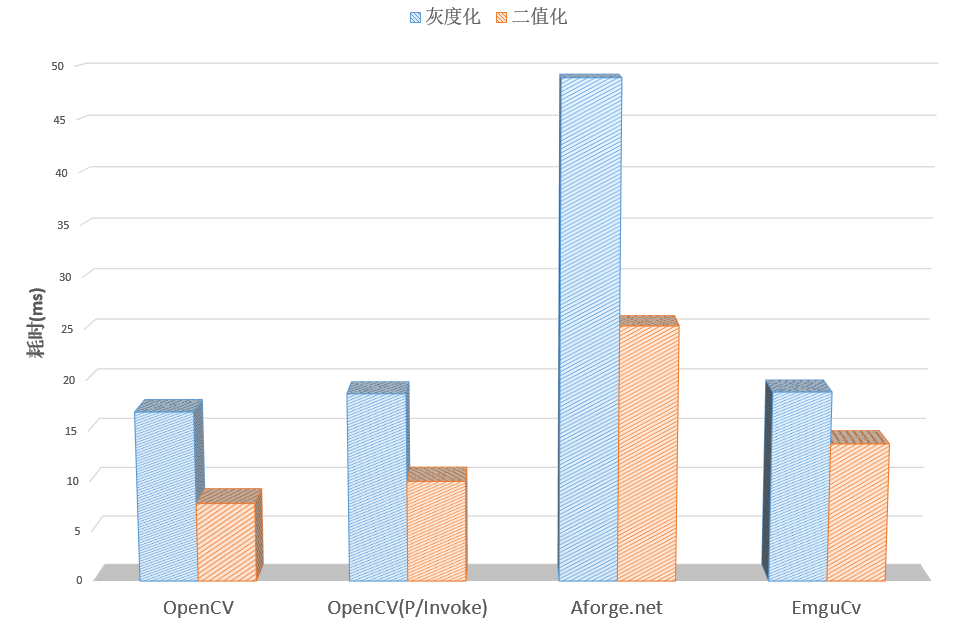
\includegraphics[width=0.9\textwidth]{Image-Processing-Comparison}
	\caption{几种图像处理库的性能比较}
	\label{pic:image-processing-comparison}
\end{figure}

OpenCV(Open Source Computer Vision)是一个旨在完成实时机器视觉(Real-time Computer Vision)的函数库,最早是由英特尔研究中心开发,后被Will Garage接手,现在是由Itseez团队负责维护,是一个跨平台的免费开源图像处理库\citep{wiki:OpenCV}。OpenCV最早于2000年发行,目前仍在更新和维护,最新的稳定版是于2015年12月发布的OpenCV 3.1更新。它的代码由C/C++写就,同时提供了Python、Java以及Matlab等语言的接口\citep{wiki:OpenCV}。自其发布后的15年来,OpenCV一直以它良好的性能和高度的稳定性著称,是使用最为广泛的图像处理库。这也意味着它有着大量的用户测试经验和成熟的社区支持,这无疑为我们解决项目中的棘手问题提供了基础保障,具体来说,本系统的数据加载模块、版面分析模块、预处理模块都需要用到OpenCV提供的函数方法支持,我们也将在后面的模块详细介绍中,体会到OpenCV的强大功能。

\subsubsection{环境部署}
OpenCV是有很好的多平台支持(Windows,Linux,Mac等),环境的部署也比较简单,这里我们仅以Windows平台下Visual Studio 2013的opencv配置使用为例,做一个部署步骤的简要展示:
\begin{itemize}
  \item 从\href{http://opencv.org/}{OpenCV官方主页}下载最新的OpenCV 3.1安装包,解压安装包完成安装。并将OpenCV加入系统环境变量。
  \item 新建一个Visual Studio C++工程,在工程配置属性中的“包含目录”中添加OpenCV的include文件夹,在“库目录”中加入OpenCV的lib文件夹,在“链接器”的附加依赖中添加opencvworld310d.lib和opencvworld310.lib(分别对应debug和release编译选项)。
  \item 在工程中添加如下测试代码OpenCV-test.cpp(代码见下方,功能是展示示例图片),编译运行,如果编译通过,并且程序正确开辟“example”窗口并显示示例图片,说明OpenCV的环境就配置成功了。
\begin{lstlisting}[label=OpenCV-test.cpp]
#include <iostream>
#include "opencv2/highgui/highgui.hpp"
using namespace cv;
int main(void)
{
  Mat img = imread("example.jpg", 0);
  imshow("example", img);
  waitKey();
  return 0;
}
\end{lstlisting}
\end{itemize}



上面只是简述了OpenCV的部署步骤,具体到不同的平台和软件版本,部署时会有一些小的差异,读者可结合自己的情况,从网络上找到对应的详细部署指南,这里就不再赘述了。

\subsection{字符识别}
\subsubsection{方案选取}
字符识别(Character Recognition),又称光学字符识别(Optical Character Recognition,OCR),是指将印刷或手写的文字转换成机器编码(machine-encoded)文本的过程,它被广泛应用于纸质印刷的数据录入中,例如护照文件、发票、信件、银行存单等,当这些纸质文件被转换成了机器编码的文本以后,无论是在编辑修改、搜索、存储,还是在后续的数据挖掘,文字转语音等过程中,都变得相对便捷和高效。OCR是模式识别(Pattern Recognition)、(Artificial Intelligence)和计算机视觉(Computer Vision)领域中的典型应用\citep{wiki:OCR}。

具体到本系统,我们是要讲光学字符识别技术应用到纸质或截图保存的病历数据中,这项技术会在OCR模块中用到,在技术实现上与其他基于光学字符识别的应用并没有本质的不同,因此我们可以采用已有的OCR解决方案。目前比较主流的OCR解决方案有ABBYY FineReader、Microsoft Office内置的OCR模块、Tesseract、FreeOCR等,维基百科中有对各种OCR软件的详细对比\citep{wiki:OCRcomparison},同时,也有组织对于最好的OCR软件做过一个排名(见\autoref{pic:ocr-software-comparison}),从这个排名中我们可以看到,好的商用OCR软件一般都售价不菲(图片中的价格仅针对个人用户),同时由于病历数据的版面结构复杂,并没有一个比较通用的版面分析方案,所以这些商用OCR软件无法直接应用到系统中,因此,我们需要一个有提供编程接口(Application Programming Interface,API)的OCR解决方案,方便定制特定场景下的OCR。能提供编程接口的OCR引擎中,Tesseract是其中的首选。

\begin{figure}
	\centering
	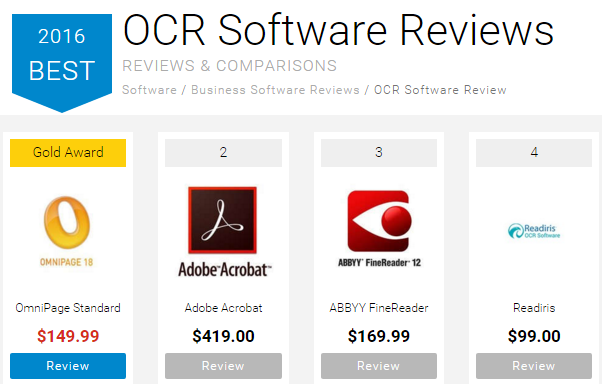
\includegraphics[width=0.9\textwidth]{ocr-software-comparison}
	\caption{某组织对现有OCR软件的排名}
	\label{pic:ocr-software-comparison}
\end{figure}

Tesseract OCR引擎是一款能运行在多系统全平台(Windows,Linux,Mac,IOS,Android)的免费开源OCR引擎,最早由惠普公司Hewlett Packard实验室的工程师在1985年到1994年间开发和维护,并于2005年开放源代码,2006年之后由谷歌公司接手开发和维护\citep{wiki:Tesseract}。

在1995年,Tesseract在识别准确率上是排名前三的OCR引擎,最早的版本只支持英文,之后逐步添加多语言的支持,其中就包括中文。准确性较高、支持多语言加之免费开源,使得Tesseract在这些年,广受赞誉,是公认最好的开源OCR引擎,读者可访问\href{https://github.com/tesseract-ocr/tesseract}{Tesseract的GitHub主页}来获取最新的源代码。同时,Tesseract的源码是由C/C++编写,与同样是C/C++编写的OpenCV图像处理库能够很好的兼容,事实上,Tesseract也开发了专门针对OpenCV的API接口,提供了丰富的支持。综上,系统决定采用Tesseract作为字符识别的解决方案。

\subsubsection{环境部署}
Tesseract支持多平台(Windows,Linux,Mac)使用和开发,如果只是简单使用tesseract,可以下载安装包安装Tesseract的可执行程序,如果需要基于Tesseract进行二次开发,则需要编译它的源代码,显然,我们的需求属于后者。接下来本文以Windows平台下Visual Studio 2013的Tesseract编译为例,做一个简要的环境部署展示:
\begin{itemize}
	\item 安装版本控制软件Git\footnote{更多相关信息可访问Git官方网站:https://git-scm.com/}。
	\item 在电脑中建立tesseract-build文件夹,在该文件夹下打开CMD控制台程序,并分别运行:
	\begin{Code}[numbers=left]
git clone git://github.com/charlesw/tesseract-vs2012.git
git clone git://github.com/tesseract-ocr/tesseract.git
	\end{Code}
	\item 打开VS 2013 Developer Command Prompt,然后输入命令:
	\begin{Code}[numbers=left]
msbuild "${tesseract-build}\tesseract-vs2012\build.proj"
	\end{Code}
	其中\$\{tesseract-build\}表示tesseract-build这个文件夹在电脑中的绝对路径。
	\item 将vs2013+64bit\_support.batch文件拷贝到tesseract-build文件夹下,然后进入到tesseract文件夹,执行以下命令:
	\begin{Code}[numbers=left]
git checkout -b 3.04-vs2013 3.04.00
git am --signoff ../vs2013+64bit_support.patch
	\end{Code}
	\item 将tesseract-build$\backslash$tesseract-vs2012$\backslash$release目录下的所有文件拷贝到tesseract-build目录下。
	\item 用VS2013打开tesseract-build$\backslash$tesseract$\backslash$vs2013下的tesseract.sln工程,开始编译,如果编译正常通过,就说明环境已经配置完成。
\end{itemize}

上面的只是一个配置过程的简述,不同平台、不同版本之间的配置方式有着比较明显的差异,需结合自身的情况,选取对应的配置部署流程,这里不再详述。

\section{数据加载模块}  %500字
在\autoref{ssec:dataLoader-design}中我们已经提到,每个病人的病历数据包含于多张图片中,那么怎么标识某张图片是属于哪个病人的呢,这就对数据的存储组织形式提出了一定的要求,可能的数据组织形式有:
\begin{itemize}
	\item 所有病人的病历图片都保存于同一个文件夹下,同一个病人的病历图片的文件名有一个相同且唯一的前缀作为该病人的标识,这样,系统就可以通过这个前缀来对病历图片进行区分,归档到同一个病人档案下。
	\item 在最外层文件夹下,每个病人都拥有一个属于自己的文件夹,文件夹内就是这个病人的所有病历图片,图片文件名则没有特别要求,这样,系统就可以通过文件夹来对病历图片进行区分,归档到同一个病人档案下。
\end{itemize}
综合考虑之后,本系统采用的是第二种方案,它的优点有:
\begin{itemize}
	\item 相比第一种方案,多了一层文件夹结构,使得数据组织更加有层次,便于管理与查看。
	\item 在数据存储时,不再需要对每张图片进行重命名增加前缀,大大减少了工作量。
\end{itemize}
除此之外,这样的数据组织形式也提供了如下功能特性:
\begin{itemize}
	\item 可添加简单的容错处理。通过检测文件夹下图片的数目,我们可以确定是否有图片缺失或是冗余,可以作为一个简单的容错处理。
	\item 忽略已归档的病历。系统可以根据文件夹名字,维护一个已归档病历数据的列表,这样,在扫描文件夹时,忽略已归档病历。
\end{itemize}
具体实现上,OpenCV中提供了读取目录下所有图片的函数,具体代码如下:
\begin{lstlisting}
int main()
{
  vector<String> filenames;
  String folder = "some_folder_path";
  glob(folder, filenames);
  for(size_t i = 0; i < filenames.size(); ++i)
  {
    Mat src = imread(filenames[i]);
    if(!src.data)
        cerr << "Problem loading image!!!" << endl;
    /* do whatever you want with your images here */
  }
}
\end{lstlisting}
其中,some\_folder\_path就是某个病人的病历文件夹名字,filenames中存储的就是文件夹底下的图片名字。

\section{版面分析模块}  % 3000字
文档版面分析(Document Layout Analysis),是指在含有文本的图像中识别出感兴趣区域(Regions of Interest,ROI)的过程。一个文字识别系统需要将文字从非文字的区域中划分出来,同时保持文本的相对顺序\citep{baird1992anatomy}。在一个文件中检测和标记出文本区域和其他非文本区域的过程叫做几何学版面分析(Geometric Layout Analysis)\citep{cattoni1998geometric}。但是不同的文本区域在文档中代表的含义并不相同,例如有些文本是文档的标题,有些是文档的注释,有些是文档的主体等等,具体到病历档案归类系统中,就是文本块所属的字段是各不相同的,这种识别文字在文档中的含义的过程叫做逻辑学版面分析(Logical Layout Analysis)\citep{haralick1994document}。

(几何学)版面分析算法总体上可以分为三类\citep{mao2003document}:
\begin{itemize}
	\item 自顶向下方法,算法从整张图片开始,迭代地将图片不断分割成更小的区域,直到程序达到某种终止条件时停止。它的优点是操作简单、速度较快,但是难以适应比较复杂的版面\citep{nagy1992prototype}\citep{baird1990image}。
	\item 自底向上方法,与自顶向下的方法相反,算法从每一个图片像素开始,根据一定的聚即规则,逐渐聚集相邻的区域形成单词,语句和段落。它的优点是能够适应比较复杂的版面,缺点是速度比较慢,难以确定一个比较好的聚集规则\citep{o1993document}\citep{kise1998segmentation}。
	\item 混合型方法,它可以被看做是自顶向下和自底向上这两种方法的混合\citep{pavlidis1992page}。
\end{itemize}

在真实的应用场景中,由于实际文档的多样性,复杂性,因此,目前还没有一个固定的,最优的切割模型,需要我们根据实际问题和需求,有针对性的设计版面分析方法。在\autoref{ssec:framework-segmentation-analysis}中我们已经提到,系统的版面分析模块非常重要,需要完成以下三大功能:
\begin{itemize}
	\item 对病历图片进行二次分类;
	\item 剔除图片中的干扰信息,获得病历数据主体;
	\item 剔除主体内容中的空白,提取出各个字段。
\end{itemize}
这三个功能我们可以简单归纳为图片分类、主体保留、字段提取。这三者的顺序是从逻辑上出发来区分的,在实际代码实现中,我们是先实现了主体保留,此时再对图片分类,最后做字段提取的工作。接下来,我们分别讨论这三个功能如何实现。

\subsection{主体保留}
图片中除了我们需要的病历主体信息以外,一般还会有冗余的干扰信息,以\autoref{pic:input-image-1}为例,图片的中间部分是病人病历数据的主体,而图片上部则是一些电子病历系统的系统信息,左侧则是一个侧边栏导航,这些都是与病历无关的,我们需要将其剔除,保留主体,这里需要用到图片的裁剪。

\subsubsection*{OpenCV中矩形框裁剪}
在OpenCV中,可以很方便的根据矩形框来裁剪,假如原始图片已转换为Mat格式\footnote{Mat是OpenCV 2.x中图片加载以后的格式},名字为origin,我们需要产生的裁剪图片为cut,那么裁剪的代码为:
\begin{Code}
cut = origin( Rect(x0, y0, width, height) );
\end{Code}
其中$(x_0,y_0)$表示裁剪区域的左上角在原图中的位置,width和height则分别表示裁剪区域的宽度和高度。

现在我们知道用OpenCV裁剪矩形图片了,但是对于\autoref{pic:input-image-1}这样的数据,我们怎么确定$(x_0,y_0)$和width、height呢?

\subsubsection*{模板匹配}
需要注意的是,在确定的病历系统中,其系统信息和侧边栏导航的内容和位置是相对固定的,我们可以根据这一点,利用模板匹配的方式,确定系统信息栏和侧边导航栏的位置,并进行裁剪。

模板匹配(Template Matching)\citep{template-matching},是一项在原始图片中寻找匹配模板图片的小区域的技术。在OpenCV中,提供了模板匹配的函数
\begin{Code}
void matchTemplate(InputArray image, InputArray templ, OutputArray result, int method)
\end{Code}
其中image表示原始图像,templ表示模板图像,result为结果矩阵,method为匹配算子类型。具体匹配过程为模板图像在原始图像中滑动,根据不同的匹配算子,计算重叠区域的匹配度,当滑动过整个原始图像区域后,返回匹配度最高的子图像信息。

OpenCV提供了6种默认的匹配算子,最常见的是平方差匹配算子(\autoref{eq:square})和相关匹配算子(\autoref{eq:correlation}):
\begin{equation} \label{eq:square}
R(x,y)=\sum_{x^{'},y^{'}}(T(x^{'},y^{'})-I(x+x^{'},y+y^{'}))^2
\end{equation}

\begin{equation} \label{eq:correlation}
R(x,y)=\sum_{x^{'},y^{'}}(T(x^{'},y^{'})\cdot I(x+x^{'},y+y^{'}))
\end{equation}
其中,$T(x^{'},y^{'})$表示模板图像中的点,$I(x+x^{'},y+y^{'})$表示原始图像滑动窗口中对应的点。平方差匹配算子衡量的是两者的差别,所以这个值越低,说明匹配度越高,而相关匹配算子衡量的是两者的相关性,所以这个值越高,说明匹配度越高。

\begin{figure}
	\centering
	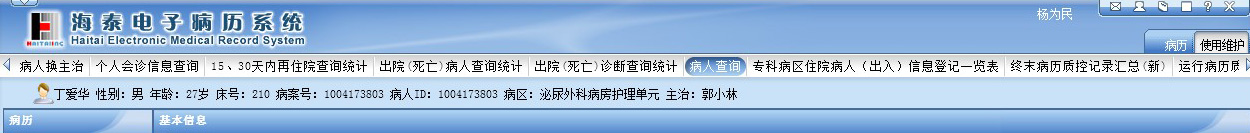
\includegraphics[width=0.9\textwidth]{title-template}
	\caption{系统信息栏模板}
	\label{pic:title-template}
\end{figure}

对于病历图片中的系统信息栏,我们可以通过截取原图中系统信息栏的部分保存下来,作为模板,如\autoref{pic:title-template}所示。然后运用模板匹配算法,剪裁掉原图中上方系统信息栏部分,代码如下:(其中算子采用平方差算子,输入参数src代表原图,\_template代表模板,template\_type为模板类型,返回值roi为截掉模板之后的图像。)
\begin{Codex}[label=Cut,numbers=left]
Mat MatchingMethod(Mat src, Mat _template, int template_type)
{
	// template_type option:  0 -> title, 1 -> sidebar
	Mat result;
	int match_method = CV_TM_SQDIFF_NORMED;
	Mat img_display;
	src.copyTo(img_display);
	int result_cols = src.cols - _template.cols + 1;
	int result_rows = src.rows - _template.rows + 1;
	result.create(result_rows, result_cols, CV_32FC1);
	matchTemplate(src, _template, result, match_method);
	normalize(result, result, 0, 1, NORM_MINMAX, -1, Mat());
	double minVal; double maxVal; Point minLoc; Point maxLoc;
	Point matchLoc;
	minMaxLoc(result, &minVal, &maxVal, &minLoc, &maxLoc, Mat());
	matchLoc = minLoc;
	Mat roi;
	if (template_type)
	roi = src(Rect(matchLoc.x + _template.cols, matchLoc.y, src.cols - matchLoc.x - _template.cols, _template.rows));
	else
	roi = src(Rect(0, matchLoc.y + _template.rows, matchLoc.x + _template.cols, src.rows - matchLoc.y - _template.rows));
	return roi;
}
\end{Codex}

去掉系统信息栏之后的图像如\autoref{pic:template-cut-title}所示,接着我们采用同样的方法,也可去掉侧边的导航栏,最终得到\autoref{pic:template-cut-title}所示,可以看到,病历的主体已经被完整的剥离出来,至此,主体保留的工作就完成了。

\begin{figure}[htbp]
  \centering
  \subfloat[]{
  \label{pic:template-cut-origin}
  \begin{minipage}[t]{0.3\textwidth}
    \centering
    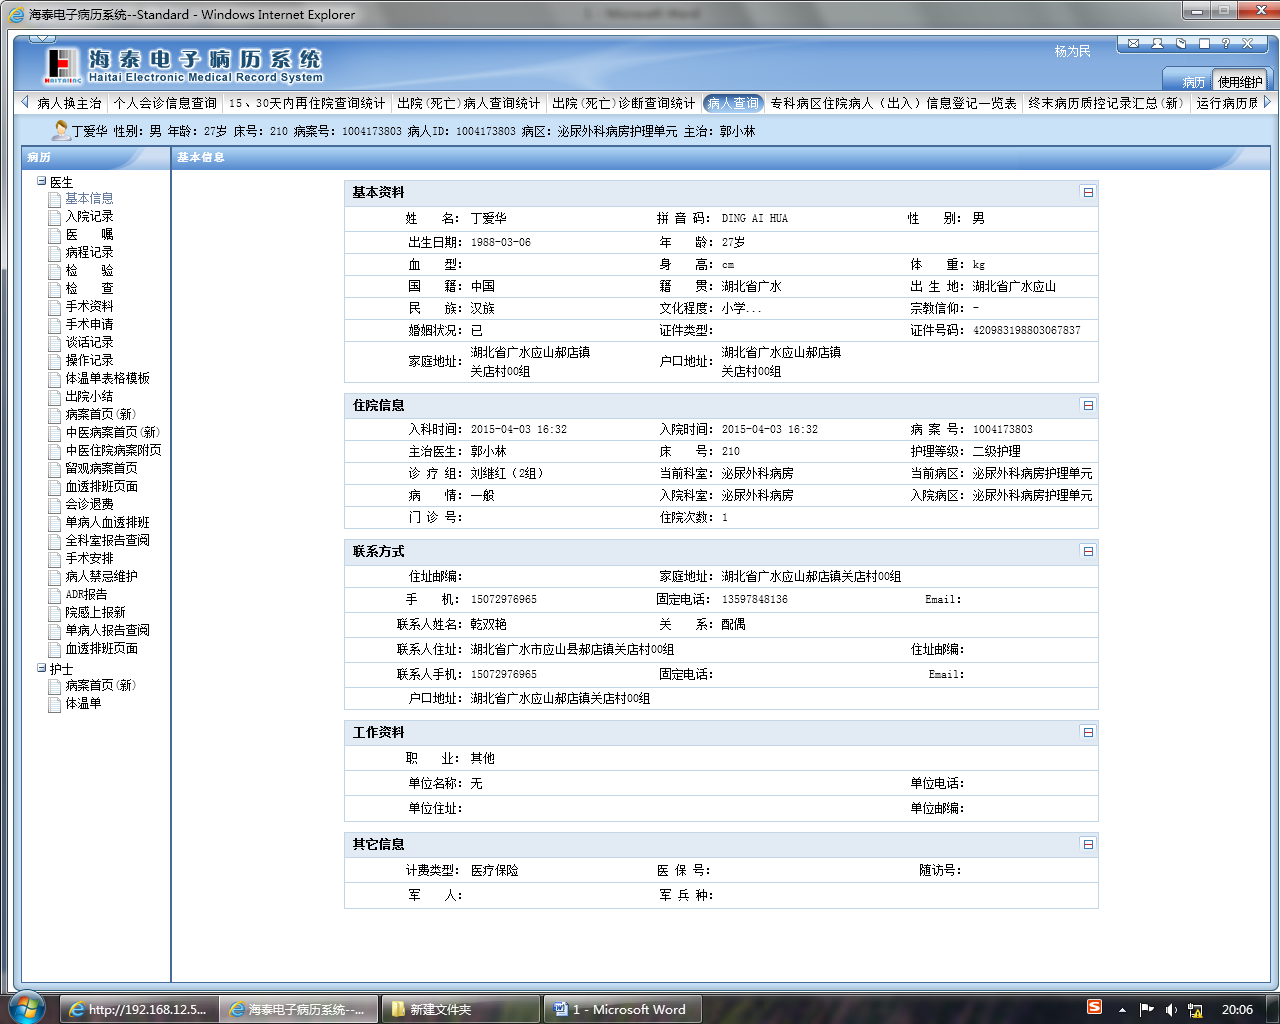
\includegraphics[width=\textwidth]{input-image-1}
  \end{minipage}
  }
  \subfloat[]{
  \label{pic:template-cut-title}
  \begin{minipage}[t]{0.3\textwidth}
    \centering
    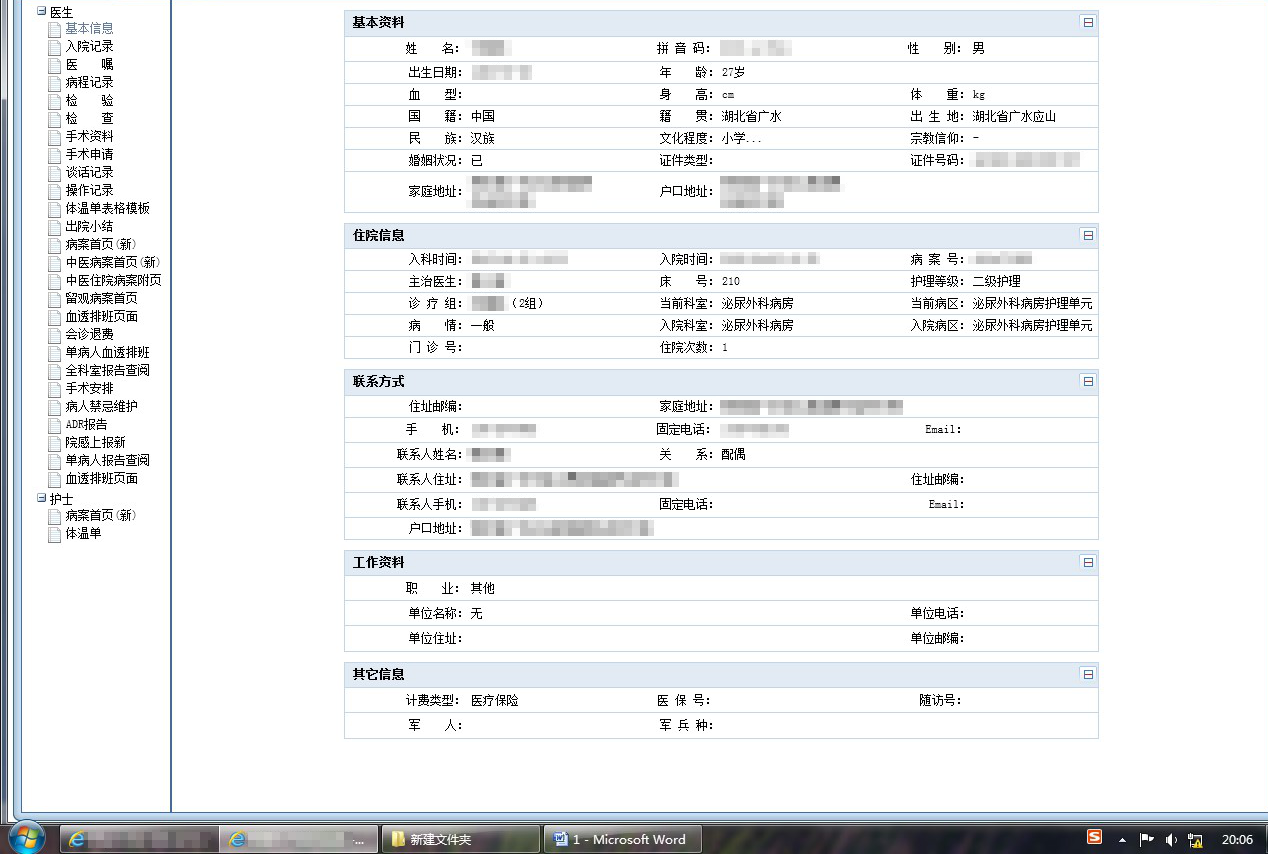
\includegraphics[width=\textwidth]{cut_title}
  \end{minipage}
  }
  \subfloat[]{
  \label{pic:template-cut-sidebar}
  \begin{minipage}[t]{0.3\textwidth}
    \centering
    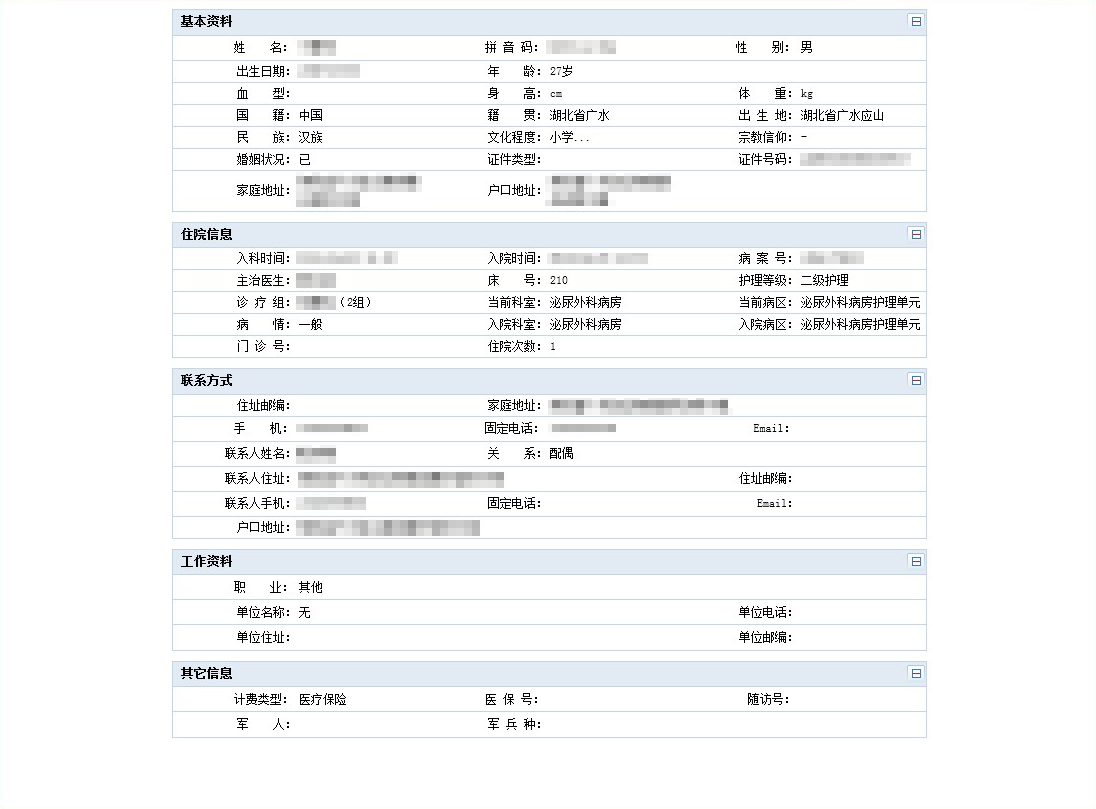
\includegraphics[width=\textwidth]{cut_sidebar}
  \end{minipage}
  }
  \caption{病历主体内容截取}
  \label{pic:different-layout}
\end{figure}

\subsection{图片分类}
在\autoref{ssec:framework-segmentation-analysis}中,我们已经提到每个病人对应着大约7到10张图片,这些图片的内容互不重复,加起来构成了完整的病人诊疗信息,图片之间的版式是各不相同的,如\autoref{pic:different-layout}所示,三张图片都属于同一个病人的病历数据,但是主体内容的版式各不相同,\autoref{fig:sub-input-image-1}中主要记录的是病人的基本信息,如姓名、性别等,\autoref{fig:sub-input-image-3}中记录的则是病人详细的病情数据,而\autoref{fig:sub-input-image-2}则介于两者之间。假设病人的病历图片只有这三种样式,那么当有一张图片输入时,应该如何判断这张图片属于哪个样式呢?这就涉及到图片相似度(image similarity measure)度量的问题了。

\begin{figure}[htbp]
  \centering
  \subfloat[]{
  \label{fig:sub-input-image-1}
  \begin{minipage}[t]{0.3\textwidth}
    \centering
    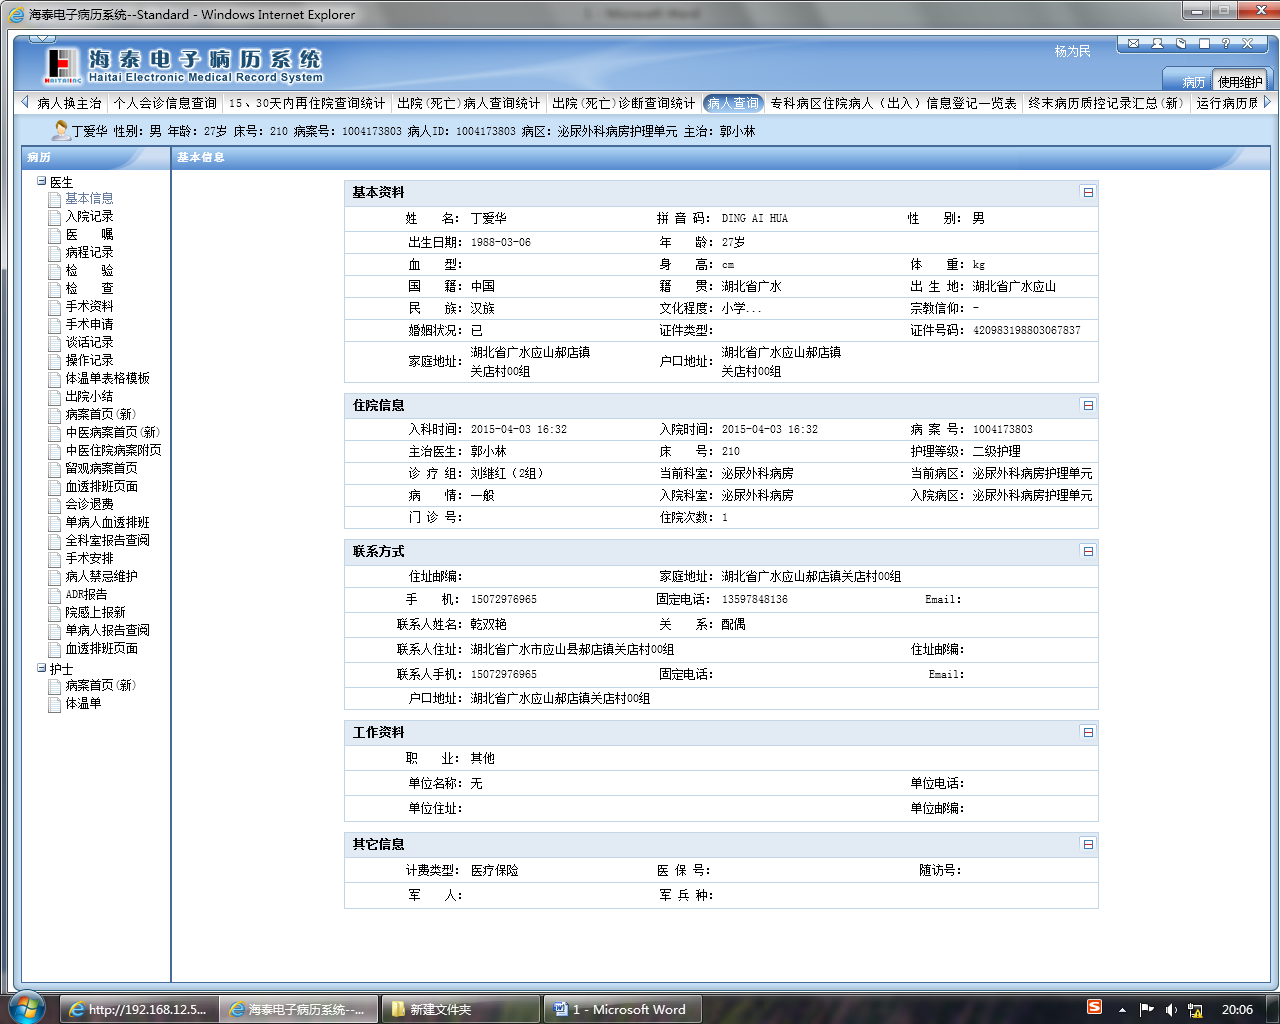
\includegraphics[width=\textwidth]{input-image-1}
  \end{minipage}
  }
  \subfloat[]{
  \label{fig:sub-input-image-2}
  \begin{minipage}[t]{0.3\textwidth}
    \centering
    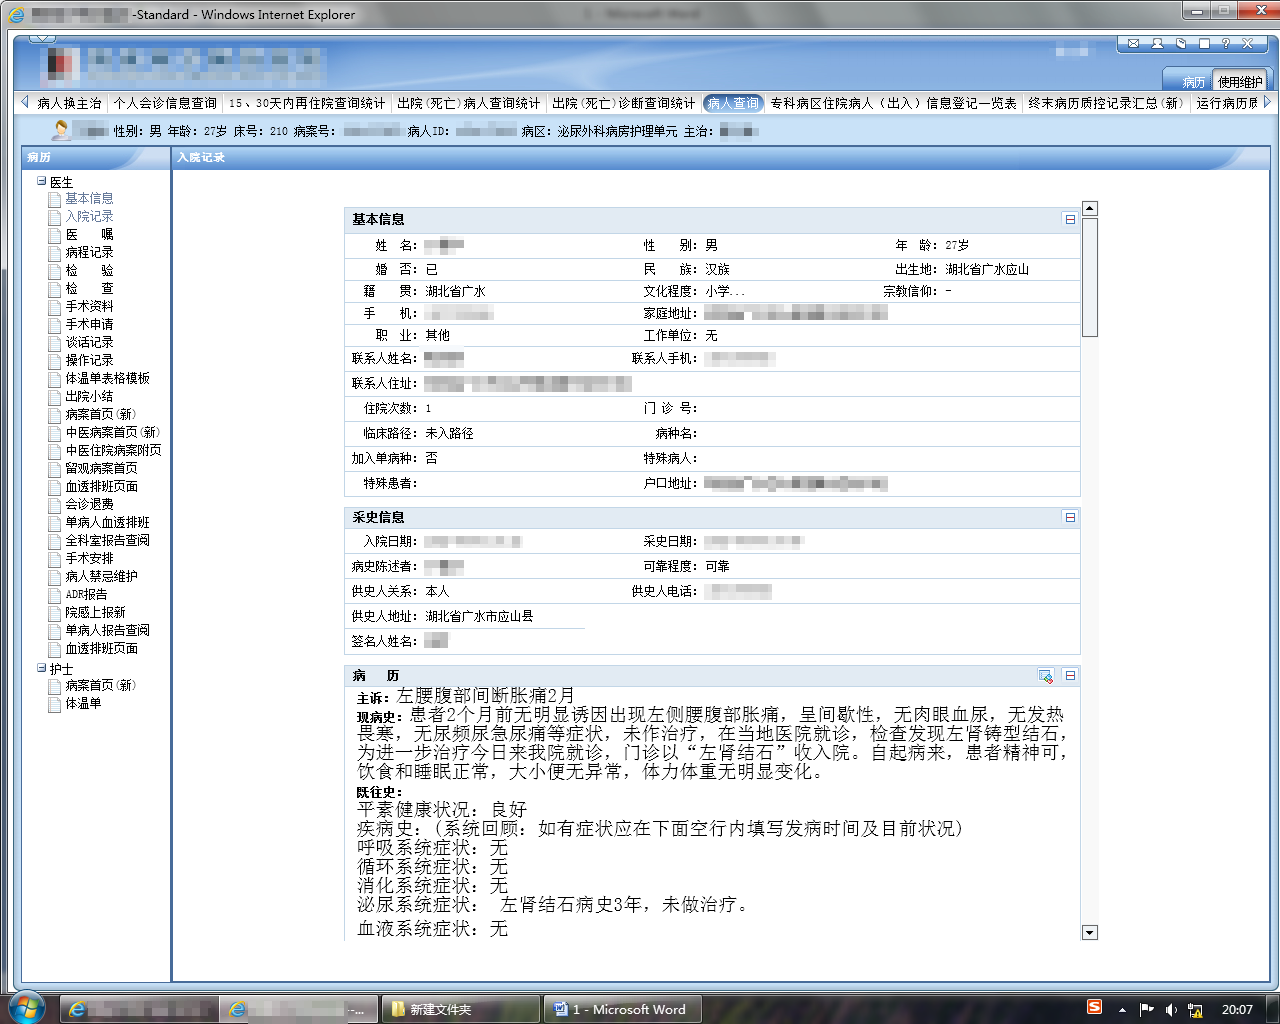
\includegraphics[width=\textwidth]{input-image-2}
  \end{minipage}
  }
  \subfloat[]{
  \label{fig:sub-input-image-3}
  \begin{minipage}[t]{0.3\textwidth}
    \centering
    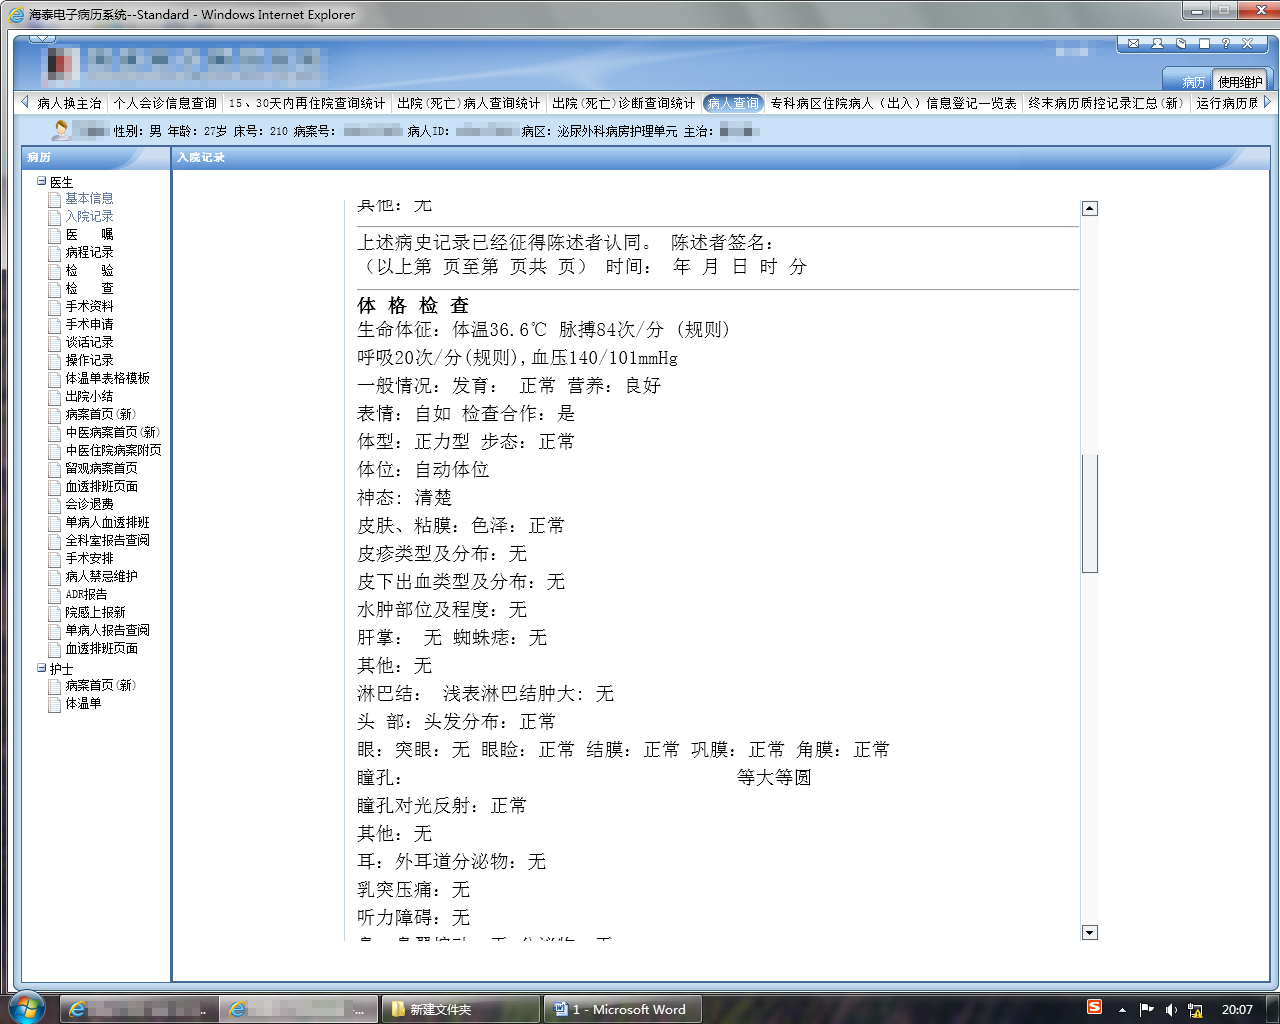
\includegraphics[width=\textwidth]{input-image-3}
  \end{minipage}
  }
  \caption{病历图片的几种版式}
  \label{pic:different-layout}
\end{figure}

相似性度量(Similarity Measure)\citep{lin1998information},或者距离度量(Distance Meature),是一个用来定义两个物体相似性或者距离的实值函数\citep{singhal2001modern},常见的相似性度量函数有欧几里得距离(Euclidean distance)\citep{wiki:Euclidean-distance}、余弦距离(Cosine Distance)\citep{wiki:Cosine-distance}、机器学习中的核函数(Kernel Functions)\citep{hofmann2008kernel}等等,这些相似性度量在数据挖掘领域有着广泛的应用\citep{tan2006introduction}。图片相似度度量,是相似性度量的一个特例,当然,版式作为图片信息的一个抽象,它的相似度度量是图片相似度度量的一个子集。一般来说,图像相似性度量分为两个部分\citep{goldberger2003efficient}:
\begin{itemize}
  \item 图像表示(Image Representation),既然相似性度量是一个实值函数,那么图片数据需要转换成某种数值的表示形式才能进行度量,比较常见的表示方法是将图片中的每个像素分成红绿蓝三个维度的0-255的整数值进行存储,而灰度、二值等都是不同的图片表示方法。
  \item 相似度定义与计算,定义一个合适的相似度度量指标,计算图片间的相似度。这个是与问题相关的,不同问题适用的相似度度量也不一样。
\end{itemize}
具体到病历图片版面相似性度量,由于我们的病历图片的版式只有固定的几种,假设为三种,这样对于每张图片,我们可以与这三种版式分别进行相似性比较,相似度最高的就是该图片的版式。但是对于同一种版式,各个字段的内容是不相同的,比如姓名字段,每个病人的名字就各不相同,因此,我们需要预先对图片做一些处理,抛弃一些细节信息,消除因为各个字段内容不同造成的整体相似度的差异。这里就需要用到图像处理中图片的灰度化、二值化、腐蚀等操作了,我们先来逐一介绍下这几种图像转换方法。

\subsubsection*{灰度化}
\label{sub:灰度化}
一张彩色图像在计算机中是由若干个像素点的形式存在,像素点的多少取决于图像的分辨率PPI(Pixel Per Inch),而每个像素点最常见的表示形式是RGB(Red,Green,Blue,即红。绿。蓝)三原色,三原色的不同组合比例能表示丰富的色彩。而灰度图(Greyscale Image)则是另外一种表示形式,它只保存了每个像素的亮度(Intensity)信息,将RGB图像转换为灰度图需满足\autoref{eq:RGBtoGray}:
\begin{equation} \label{eq:RGBtoGray}
		\begin{split}
& P(x,y) = \alpha R(x,y) + \beta G(x,y) + \gamma B(x,y),  \\
& where \quad \alpha,\beta,\gamma > 0,\alpha + \beta + \gamma = 1
		\end{split}
\end{equation}
其中,$P(x,y)$表示像素点的灰度值,$R(x,y),G(x,y),B(x,y)$表示像素点的三原色值,系数$\alpha,\beta,\gamma$的一个常见取值为$\alpha=0.299,\beta=0.587,\gamma=0.114$。从\autoref{eq:RGBtoGray}中我们可以知道,灰度转换实际上是从RGB三维到灰度一维的投影,这种转换会损失信息,并且是不可逆的。\autoref{pic:greyscale}展示了RGB图像灰度化以后的结果。

\begin{figure}[htbp]
  \centering
  \subfloat[]{
  \label{pic:lena}
  \begin{minipage}[t]{0.45\textwidth}
    \centering
    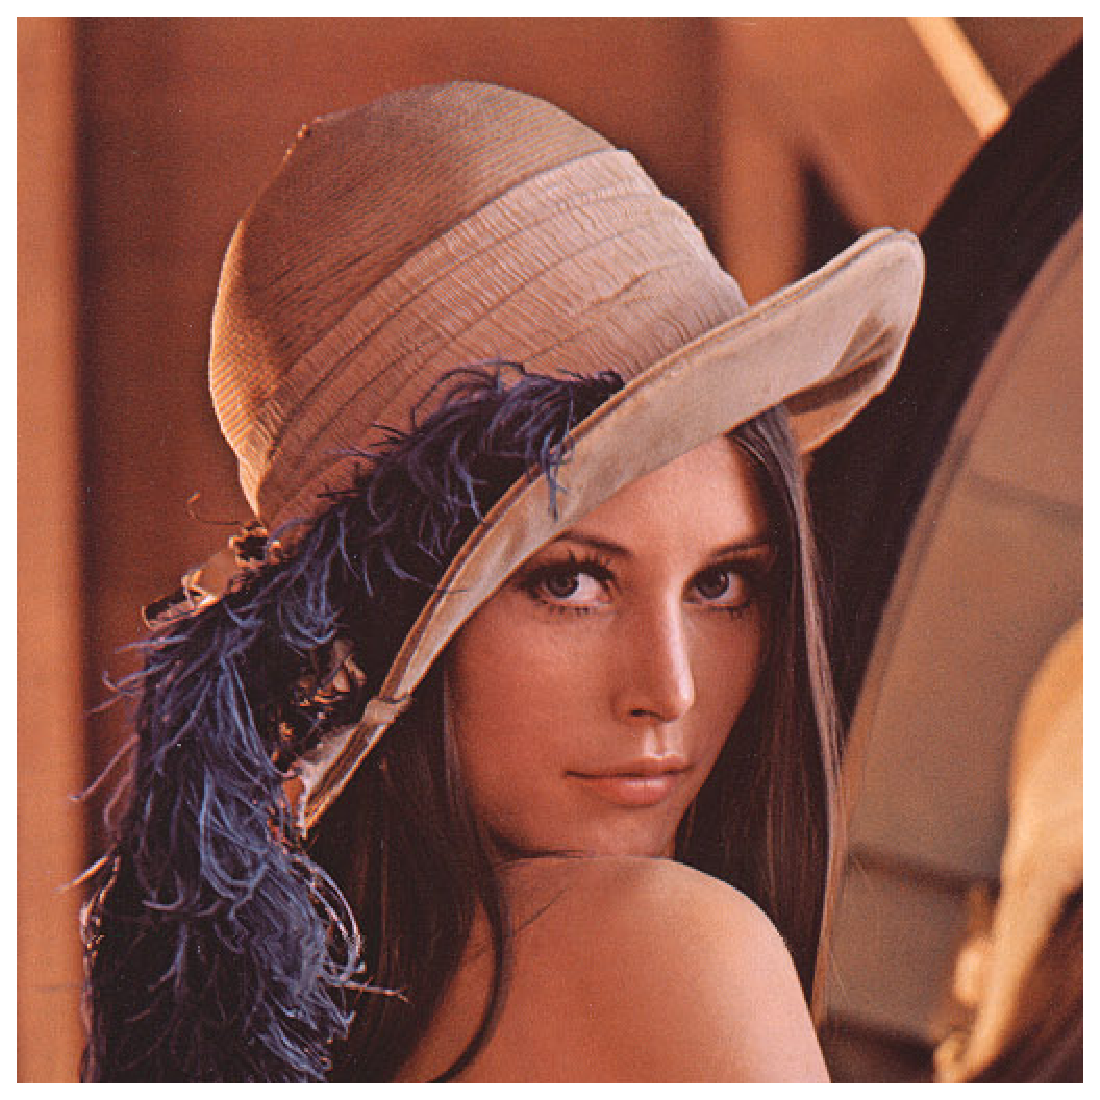
\includegraphics[width=\textwidth]{lena}
  \end{minipage}
  }
	\hfill
  \subfloat[]{
  \label{pic:lena-grey}
  \begin{minipage}[t]{0.45\textwidth}
    \centering
    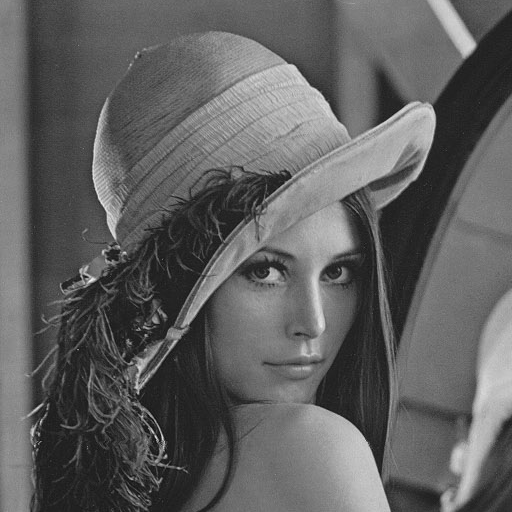
\includegraphics[width=\textwidth]{lena_grey}
  \end{minipage}
  }
  \caption{图片的灰度化}
  \label{pic:greyscale}
\end{figure}

\subsubsection*{二值化}
\label{sub:二值化}
二值化图像(Binary Image)中,每个像素只有两种可能的值,分别是黑和白,将灰度图二值化的过程满足\label{pic:binarization}:
\begin{equation} \label{pic:binarization}
	B(x)=
	\begin{cases}
		0,&x\geq threshold\cr 1,&x<threshold
	\end{cases}
\end{equation}
其中$x$表示像素点的灰度值(常见取值为$0-255$),$threshold$为二值化的阈值,当$x$大于阈值时,该像素点为白色,反之为黑色。OpenCV提供了两种二值化方法,分别是固定阈值方法和自适应阈值方法。

固定阈值方法,即需要事先指定一个全局阈值,根据这个阈值对灰度图进行二值化,函数原型为
\begin{Code}
double threshold(InputArray src, OutputArray dst, double thresh, double maxval, int type)
\end{Code}
固定阈值方法虽然实现简单,但是阈值需要人工选取,很难保证效果,当阈值选的太大时,会产生很多噪声,淹没主体(见\autoref{lena_binary_130}),阈值选的太小时,又会丢失大量的细节(见\autoref{lena_binary_70}),因此这种方法在具体实施时并不推荐。

自适应阈值方法,函数原型为
\begin{Code}
void adaptiveThreshold(InputArray src, OutputArray dst, double maxValue, int adaptiveMethod, int thresholdType, int blockSize, double C)
\end{Code}
它根据像素的邻域块的像素值分布来确定该像素位置上的二值化阈值。这样做的好处在于每个像素位置处的二值化阈值不是固定不变的,而是由其周围邻域像素的分布来决定的。亮度较高的图像区域的二值化阈值通常会较高,而亮度较低的图像区域的二值化阈值则会相适应地变小。不同亮度、对比度、纹理的局部图像区域将会拥有相对应的局部二值化阈值。常用的局部自适应阈值有:1)局部邻域块的均值;2)局部邻域块的高斯加权和。%这一段摘自http://blog.csdn.net/icvpr/article/details/8515596
自适应阈值二值化效果见\autoref{lena_binary_adaptive},图片即保证了主体的明确,没有很多噪声,又保留了大部分的细节。

\begin{figure}[htbp]
  \centering
  \subfloat[]{
  \label{pic:lena_binary_origin}
  \begin{minipage}[t]{0.45\textwidth}
    \centering
    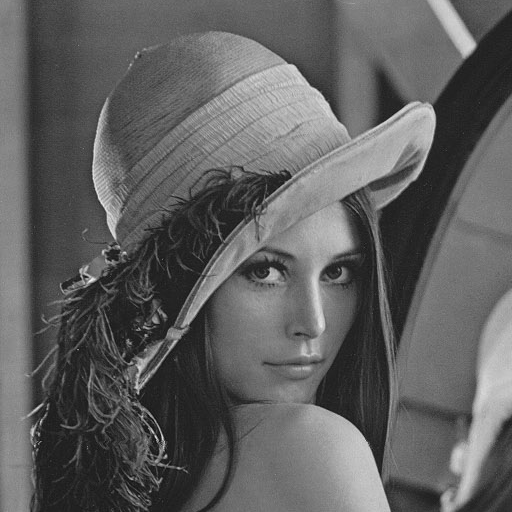
\includegraphics[width=\textwidth]{lena_grey}
  \end{minipage}
  }
	\hfill
  \subfloat[]{
  \label{pic:lena_binary_130}
  \begin{minipage}[t]{0.45\textwidth}
    \centering
    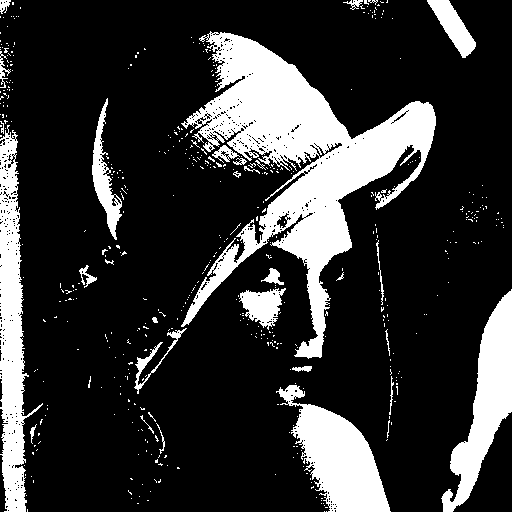
\includegraphics[width=\textwidth]{lena_binary_130}
  \end{minipage}
  }
	\vskip\baselineskip
  \subfloat[]{
  \label{pic:lena_binary_70}
  \begin{minipage}[t]{0.45\textwidth}
    \centering
    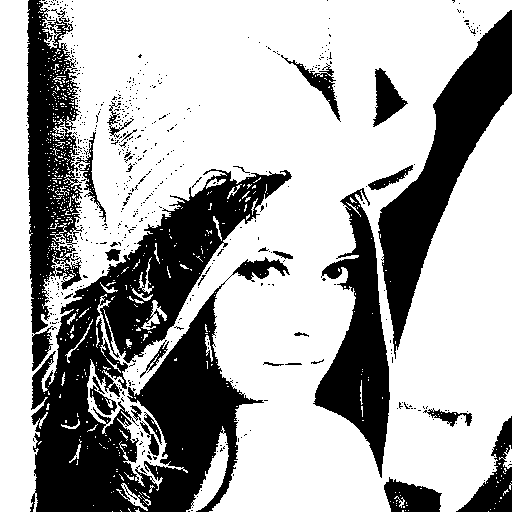
\includegraphics[width=\textwidth]{lena_binary_70}
  \end{minipage}
  }
	\hfill
  \subfloat[]{
  \label{pic:lena_binary_adaptive}
  \begin{minipage}[t]{0.45\textwidth}
    \centering
    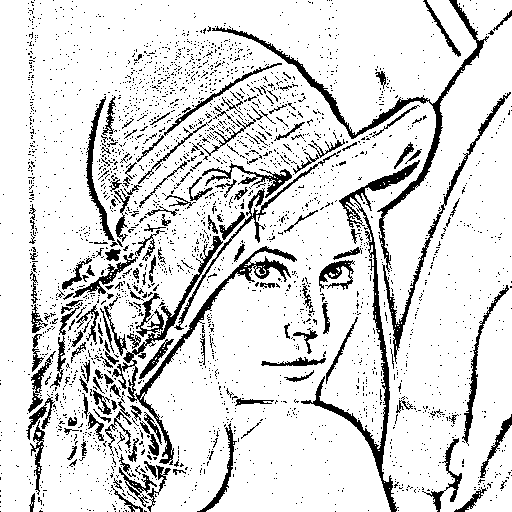
\includegraphics[width=\textwidth]{lena_binary_adaptive}
  \end{minipage}
  }
  \caption{不同二值化方法的差别}
  \label{pic:different-binary-approach}
\end{figure}

\subsubsection*{图像的膨胀和腐蚀}
图像的膨胀和腐蚀是两种常见的图像形态学操作(Morphological Operations),形态学操作简而言之,就是根据一个结构化元素(Structuring Element)对输入图片进行一系列基于外形的图像处理操作,得到输出图片。图像的膨胀和腐蚀在很多方面都有应用,例如去噪、个体元素提取或连接等。

膨胀(Dilation),可以被看做一个是基于某个核(Kernel)$B$的卷积(convoluting)操作,这个核$B$可以是任意的形状和大小,一般来说是方形或者是原型,
核$B$一般有一个预先定义好的锚点(anchor point),一般来说是核的中心。当核$B$依次扫过图片的时候,在$B$与图片的重叠区域,算法会计算区域内的最大值,并将当前锚点的值替换为这个最大值,显然,这样的最大化操作会使图片中比较亮的区域扩张,如\autoref{pic:dangan}中,\autoref{pic:dangan_origin}是包含有“档案”两个字的原图,\autoref{pic:dangan_dilated}则是经过膨胀操作以后的效果。

腐蚀(Erosion),则可以被认为是膨胀的“反操作”,即当核$B$扫过原图时,将锚点的值替换为重叠区域的最小值,这种最小化操作会使图片中比较亮的区域收缩,对应的暗色区域扩展,图片的腐蚀效果可见\autoref{pic:dangan_eroded}。

\begin{figure}[htbp]
  \centering
  \subfloat[]{
  \label{pic:dangan_origin}
  \begin{minipage}[t]{0.3\textwidth}
    \centering
    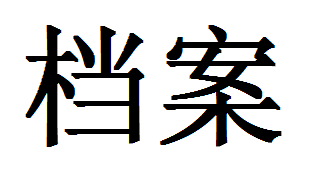
\includegraphics[width=\textwidth]{dangan_origin}
  \end{minipage}
  }
  \subfloat[]{
  \label{pic:dangan_dilated}
  \begin{minipage}[t]{0.3\textwidth}
    \centering
    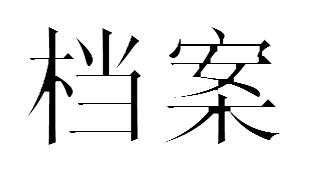
\includegraphics[width=\textwidth]{dangan_dilated}
  \end{minipage}
  }
  \subfloat[]{
  \label{pic:dangan_eroded}
  \begin{minipage}[t]{0.3\textwidth}
    \centering
    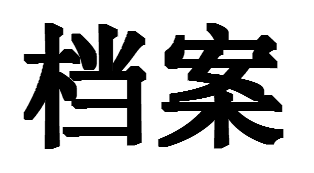
\includegraphics[width=\textwidth]{dangan_eroded}
  \end{minipage}
  }
  \caption{图片的膨胀和腐蚀}
  \label{pic:dangan}
\end{figure}

对图片的灰度化、二值化、膨胀和腐蚀操作有所了解以后,我们就可以利用这些图像处理方法,来进行图片分类任务了。前面我们提到我们是通过比较图片与三种版式图片的相似性来确定图片的版式,如\autoref{pic:layout-comparison}中所示,\autoref{pic:bingli1-cut}、\autoref{pic:bingli2-cut}、\autoref{pic:bingli3-cut}分别是保留主体的模板版式,而\autoref{pic:new-bingli1-cut}则是需要确定版式的新图片,我们只需要确定新图片与三张模板版式图片哪张最接近,就可以确定新图片的版式了。以我们的肉眼判断,测试图片的版式与\autoref{pic:bingli1-cut}是最接近的,但是,对于计算机来说,并不是那么容易判断。
\begin{figure}[htbp]
  \centering
  \subfloat[版式1]{
  \label{pic:bingli1-cut}
  \begin{minipage}[t]{0.23\textwidth}
    \centering
    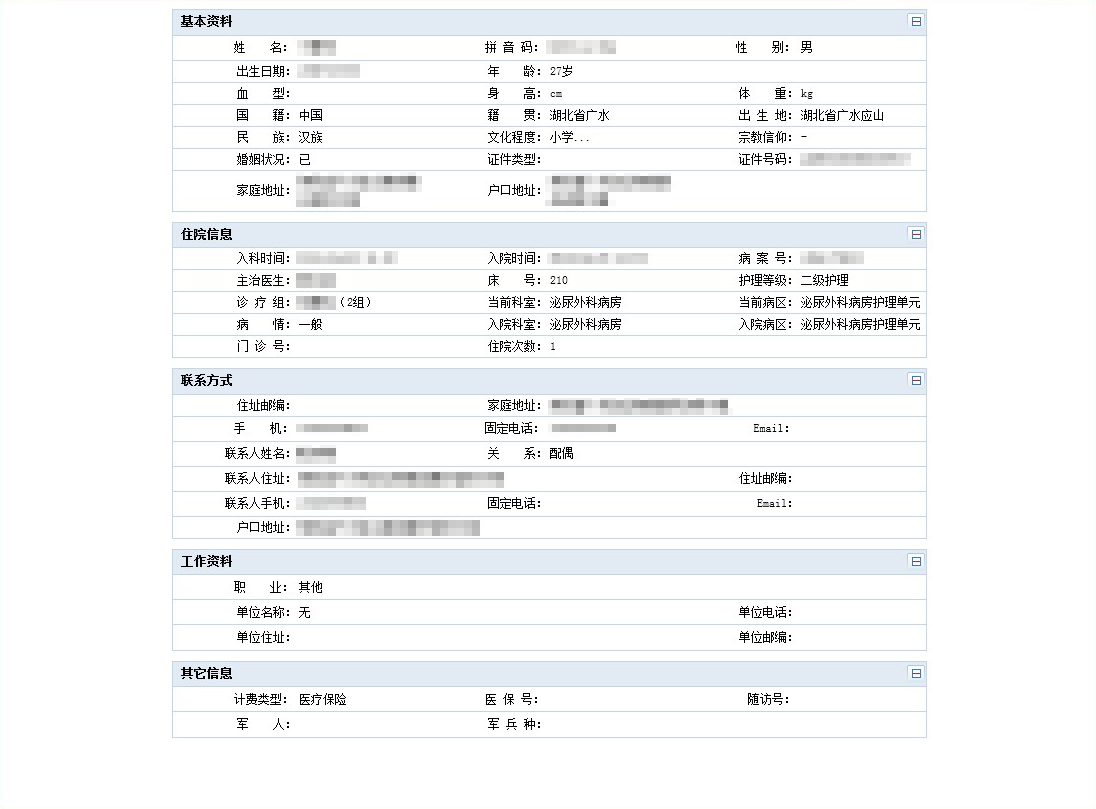
\includegraphics[width=\textwidth]{cut_sidebar}
  \end{minipage}
  }
	\hfill
  \subfloat[版式2]{
  \label{pic:bingli2-cut}
  \begin{minipage}[t]{0.23\textwidth}
    \centering
    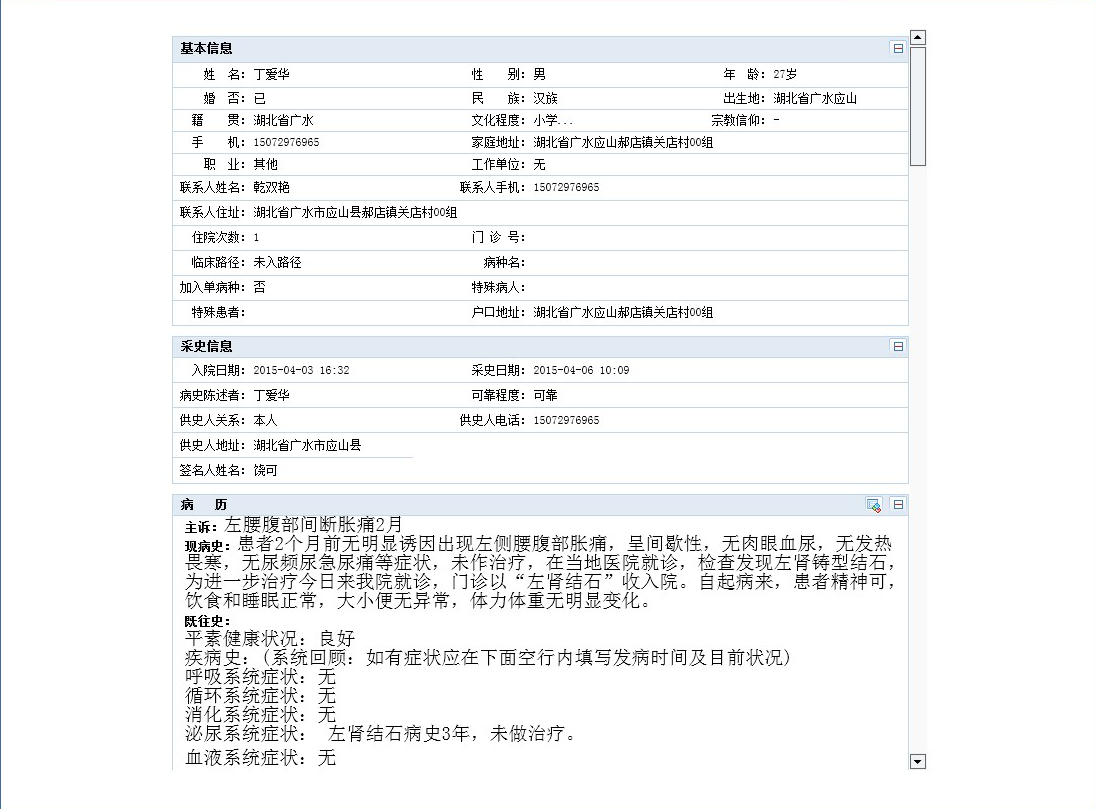
\includegraphics[width=\textwidth]{bingli2-cut}
  \end{minipage}
  }
  \subfloat[版式3]{
  \label{pic:bingli3-cut}
  \begin{minipage}[t]{0.23\textwidth}
    \centering
    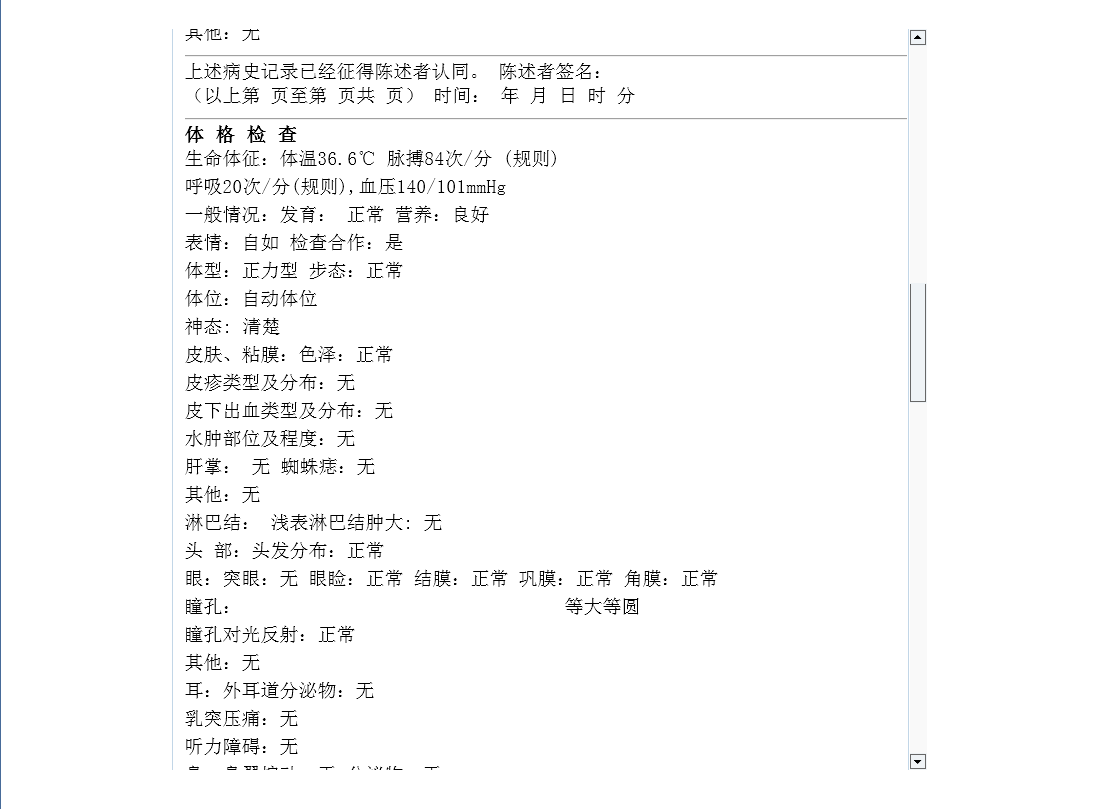
\includegraphics[width=\textwidth]{bingli3-cut}
  \end{minipage}
  }
	\hfill
  \subfloat[测试图]{
  \label{pic:new-bingli1-cut}
  \begin{minipage}[t]{0.23\textwidth}
    \centering
    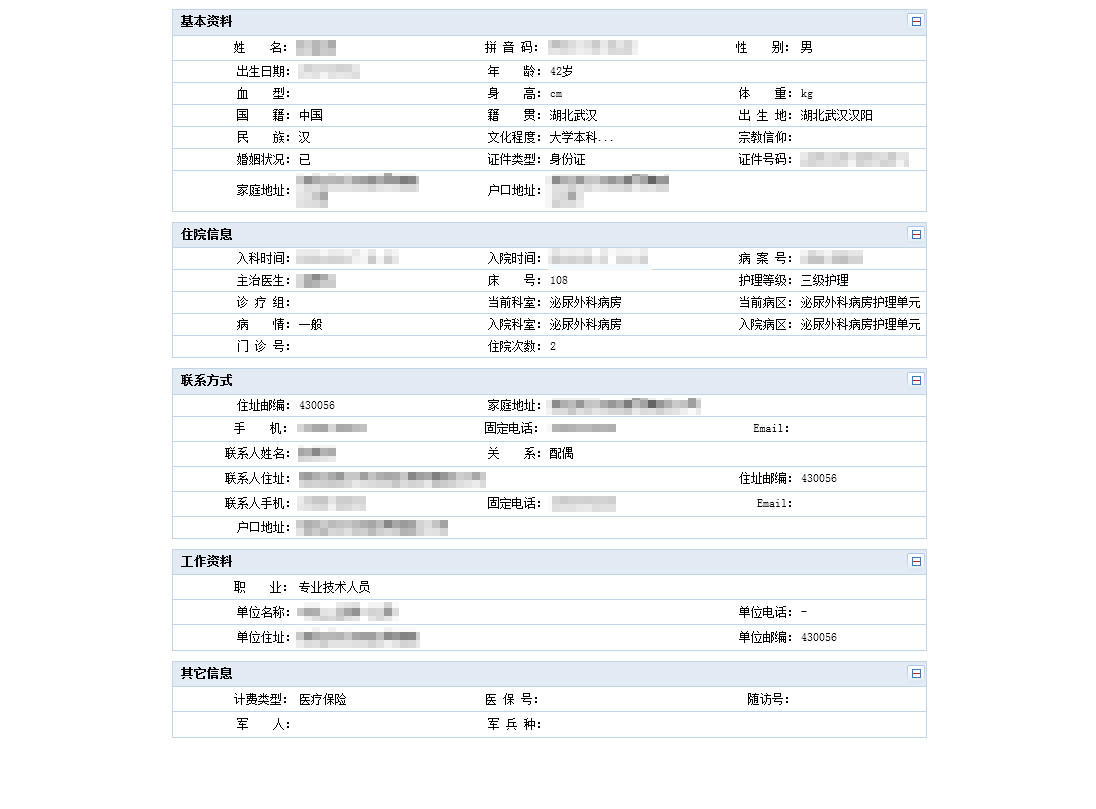
\includegraphics[width=\textwidth]{new-bingli1-cut}
  \end{minipage}
  }
	\vskip\baselineskip
  \subfloat[变换后的版式1]{
  \label{pic:bingli1-cut-eroded}
  \begin{minipage}[t]{0.23\textwidth}
    \centering
    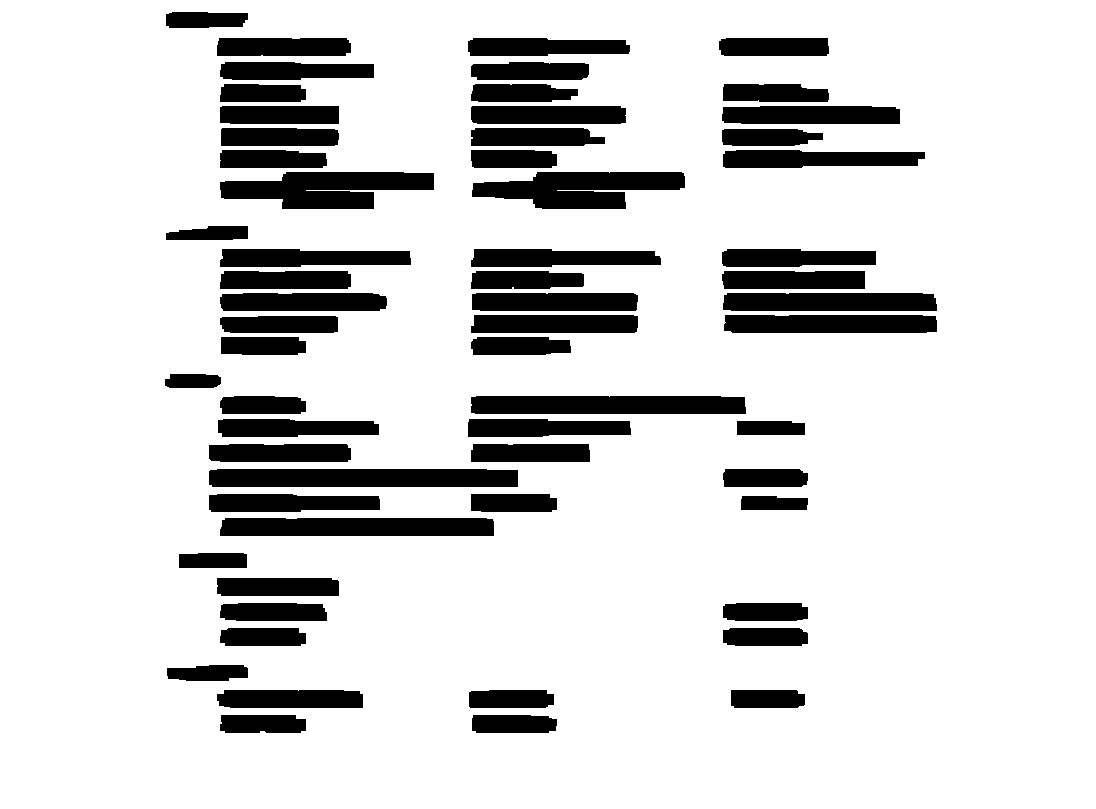
\includegraphics[width=\textwidth]{bingli1-cut-eroded}
  \end{minipage}
  }
	\hfill
  \subfloat[变换后的版式2]{
  \label{pic:bingli2-cut-eroded}
  \begin{minipage}[t]{0.23\textwidth}
    \centering
    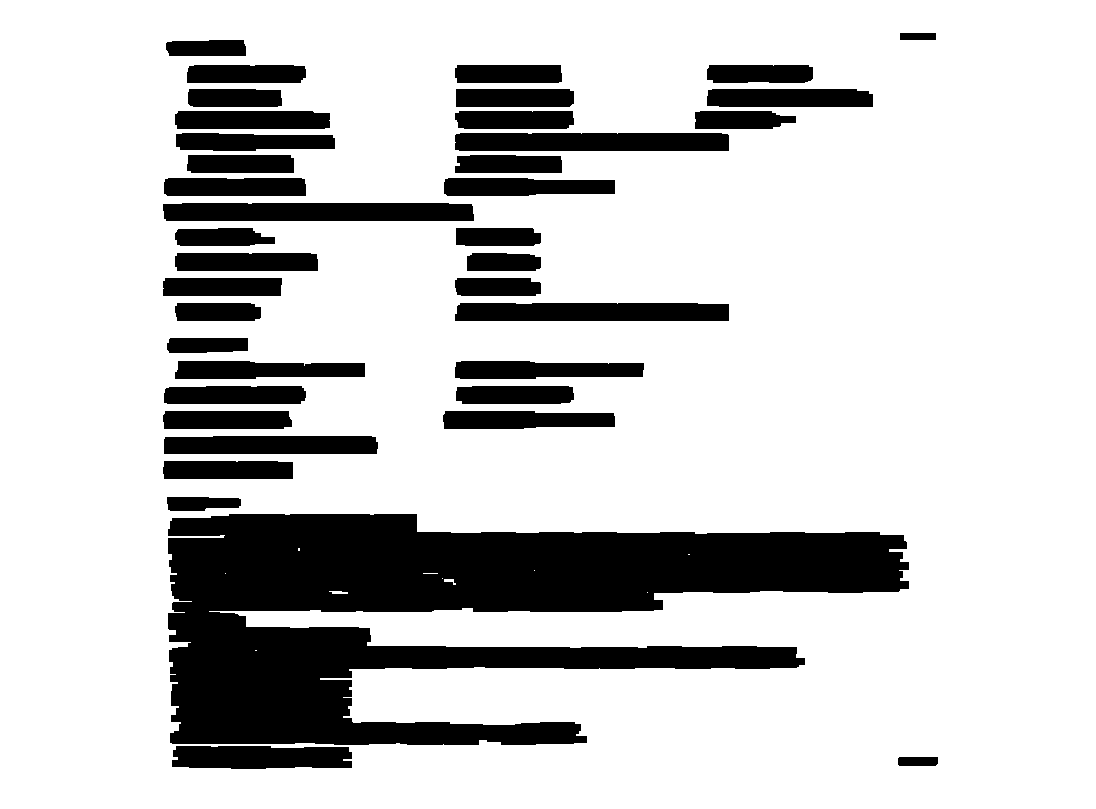
\includegraphics[width=\textwidth]{bingli2-cut-eroded}
  \end{minipage}
  }
  \subfloat[变换后的版式3]{
  \label{pic:bingli3-cut-eroded}
  \begin{minipage}[t]{0.23\textwidth}
    \centering
    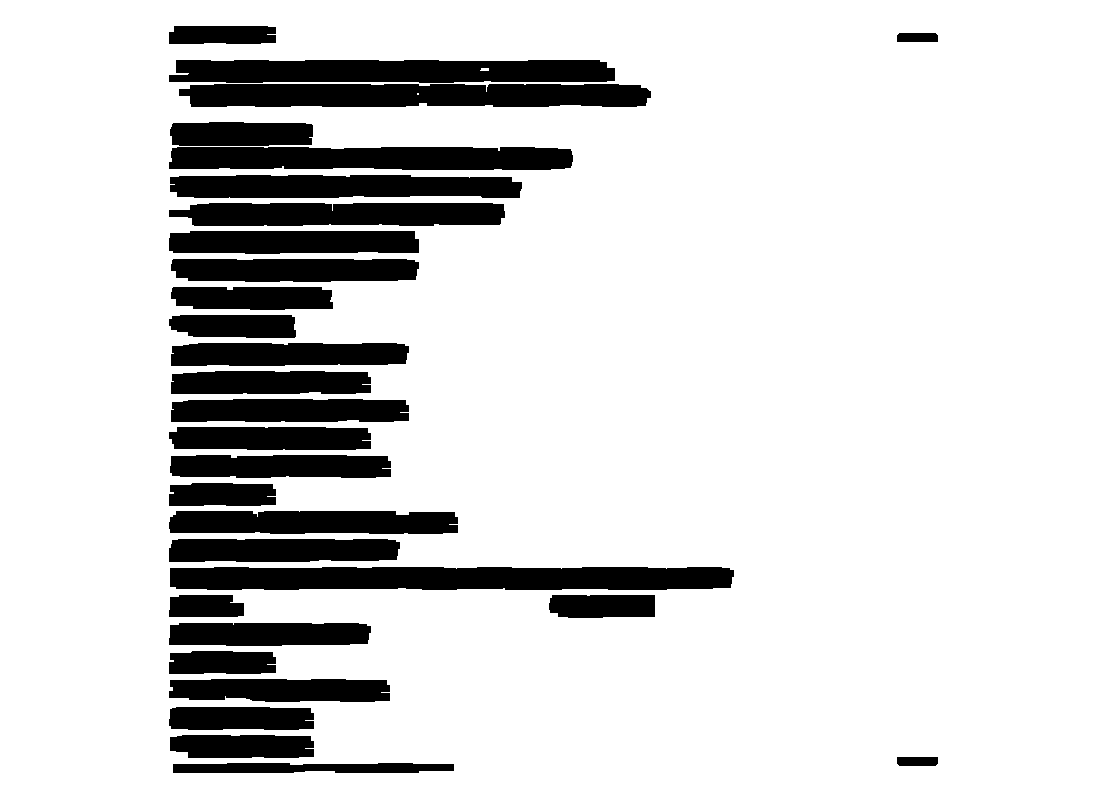
\includegraphics[width=\textwidth]{bingli3-cut-eroded}
  \end{minipage}
  }
	\hfill
  \subfloat[变换后的测试图]{
  \label{pic:new-bingli1-cut-eroded}
  \begin{minipage}[t]{0.23\textwidth}
    \centering
    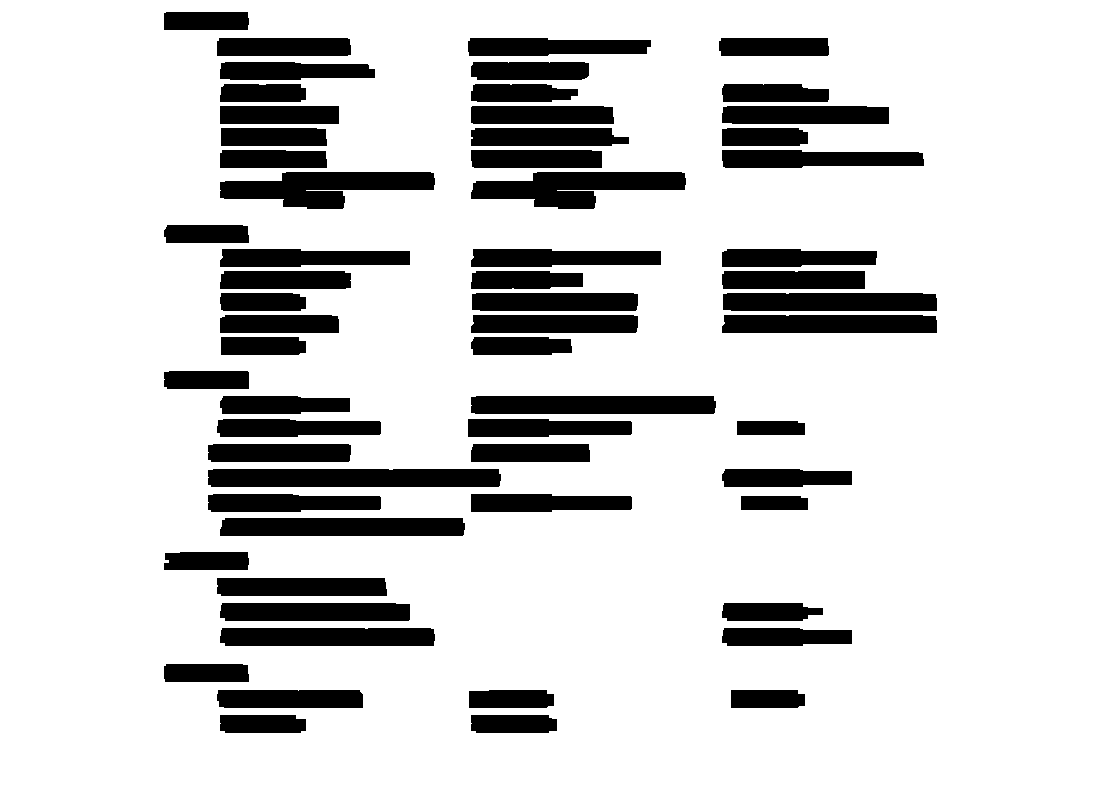
\includegraphics[width=\textwidth]{new-bingli1-cut-eroded}
  \end{minipage}
  }
  \caption{测试图片与模板图片的比较}
  \label{pic:layout-comparison}
\end{figure}

此时,这四张图片的信息比较复杂,字段中的文字实际上是判断版式的噪声,因此,我们将每张图片分别进行灰度化、二值化、腐蚀等转换操作,得到对应的\autoref{pic:bingli1-cut-eroded}、\autoref{pic:bingli2-cut-eroded}、\autoref{pic:bingli3-cut-eroded}、\autoref{pic:new-bingli1-cut-eroded}。经过转换后,图片都被二值化,即图片中的像素值只有0和1两种可能,0代表黑色,1代表白色。

每张图片我们都可以看成是一个矩阵,矩阵中的每个值要么是0,要么是1,我们采用的相似性度量指标为两张图(即两个矩阵)的点乘,显然,点乘的结果越大,说明两个图片中对应像素同时为1的像素点越多,也就可以认为越相似,点乘结果如\autoref{tab:dot-multy}所示,测试图片与版式1的点乘结果最大,因此可以认为测试图片的版式就是版式1。
\begin{table}
	\tabcaption{测试图与版式图的点乘结果}
	\label{tab:dot-multy}
	\centering
	\vspace{10pt}
  \renewcommand\arraystretch{1.5}  %这两行代码用来调整表格高度
	\begin{tabular}{|c||c|c|c|}
		\hline
		&版式1&版式2&版式3\\
		\hline
		点乘结果&$1.43\times 10^{11}$&$1.19\times 10^{11}$&$1.26\times 10^{11}$\\
		\hline
	\end{tabular}
\end{table}

但是我们可以看到,测试图片与各种版式的点乘结果间差距其实并不大,这样的判断指标显示不够有说服力,是什么原因造成点乘结果差距不明显呢?我们注意到,点乘结果主要计算的是对应像素同为1时的像素个数,即同时为白色的像素个数,而病历图片的大部分都被白色覆盖,导致点乘后,各个结果都比较接近,因此,我们可以将版式图片和测试图片的颜色都进行反转,即黑变白,白变黑,这样,点乘考量的就主要是图片中黑色相重叠的部分了。反转以后的点乘结果如\autoref{tab:dot-multy-reverse}所示,测试图片仍然是与版式1最接近,不过这一次,点乘结果间的差距更大了,这显然让我们更好做判断。

\begin{table}
	\tabcaption{测试图与版式图的反转点乘结果}
	\label{tab:dot-multy-reverse}
	\centering
	\vspace{10pt}
  \renewcommand\arraystretch{1.5}  %这两行代码用来调整表格高度
	\begin{tabular}{|c||c|c|c|}
		\hline
		&版式1&版式2&版式3\\
		\hline
		反转点乘结果&$2.62\times 10^{10}$&$1.04\times 10^{10}$&$0.95\times 10^{10}$\\
		\hline
	\end{tabular}
\end{table}

至此,我们已经完成了一张图片与版式图片之间的匹配,找到了最接近的版式,这也就意味着我们的图片分类工作完成了。

\subsection{字段提取}
接下来是版面分析的最后一步,字段提取。待分析的图片如\autoref{pic:bingli1_contours_origin}所示,我们观察可知,图片中每个字段相对于其他字段都有一定的距离,这使我们很自然的想到的通过连通域分析方法来进行字段提取工作。
\begin{figure}[htbp]
  \centering
  \subfloat[]{
  \label{pic:bingli1_contours_origin}
  \begin{minipage}[t]{0.3\textwidth}
    \centering
    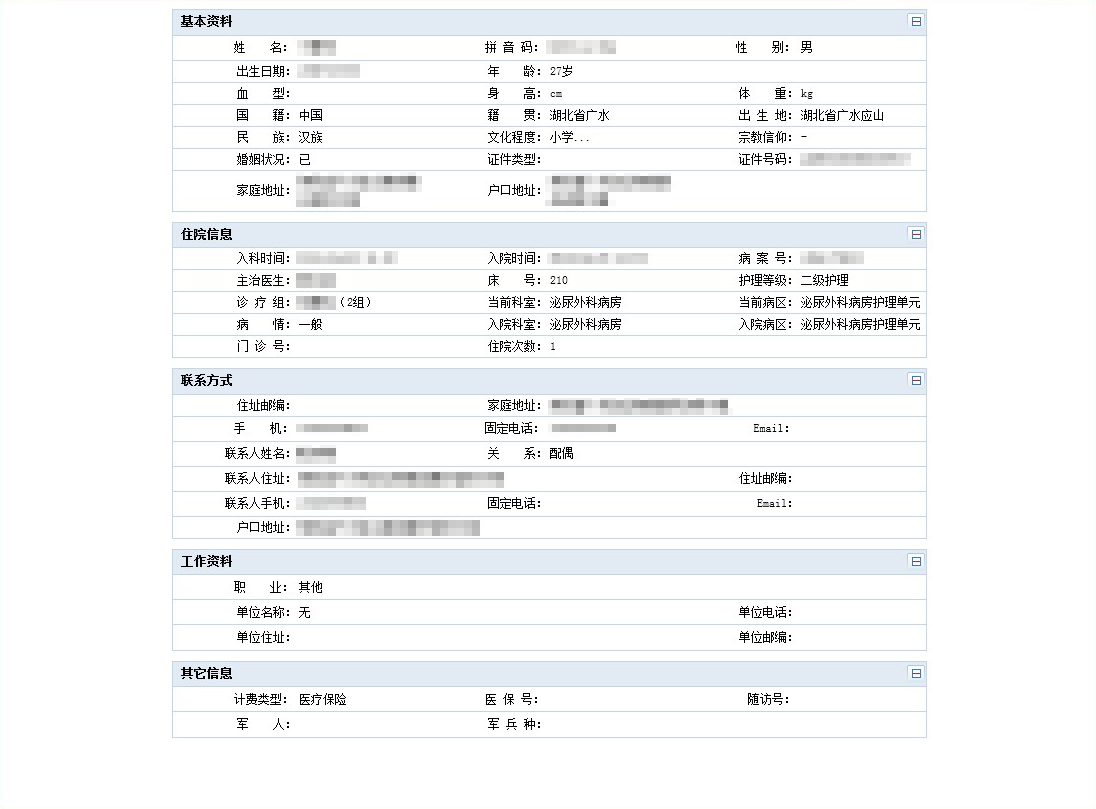
\includegraphics[width=\textwidth]{cut_sidebar}
  \end{minipage}
  }
  \subfloat[]{
  \label{pic:bingli1_contours_eroded}
  \begin{minipage}[t]{0.3\textwidth}
    \centering
    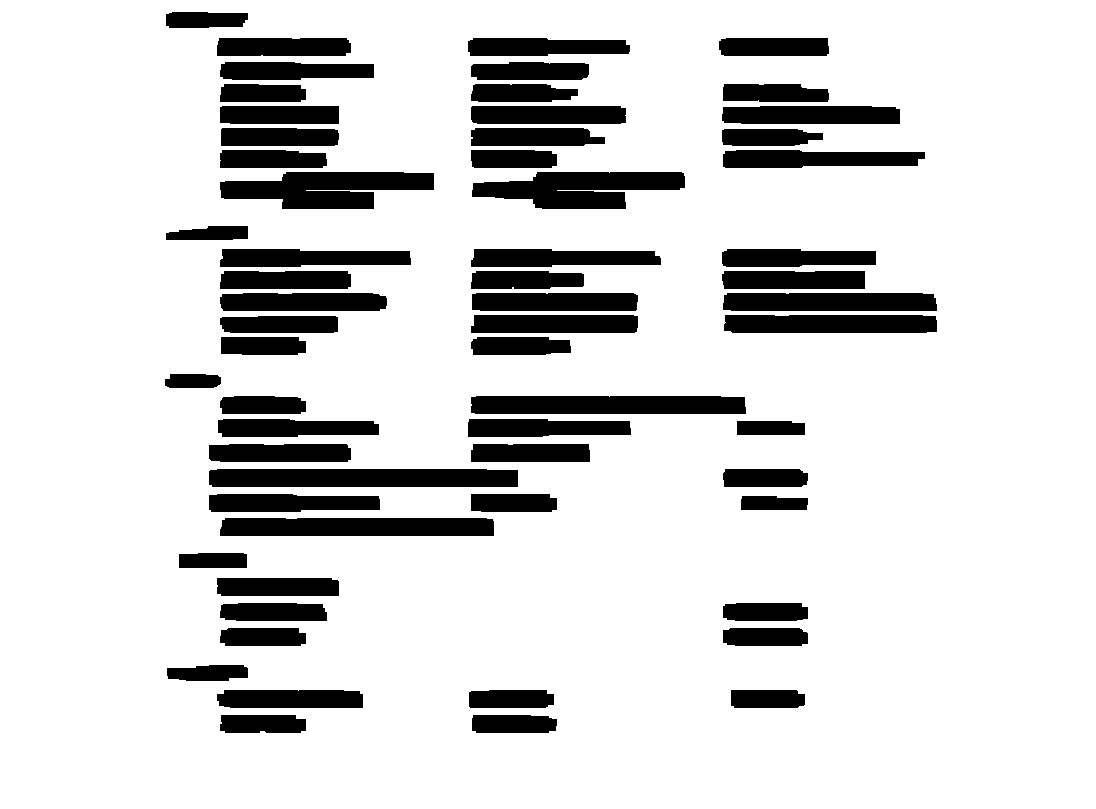
\includegraphics[width=\textwidth]{bingli1-cut-eroded}
  \end{minipage}
  }
  \subfloat[]{
  \label{pic:bingli1_contours}
  \begin{minipage}[t]{0.3\textwidth}
    \centering
    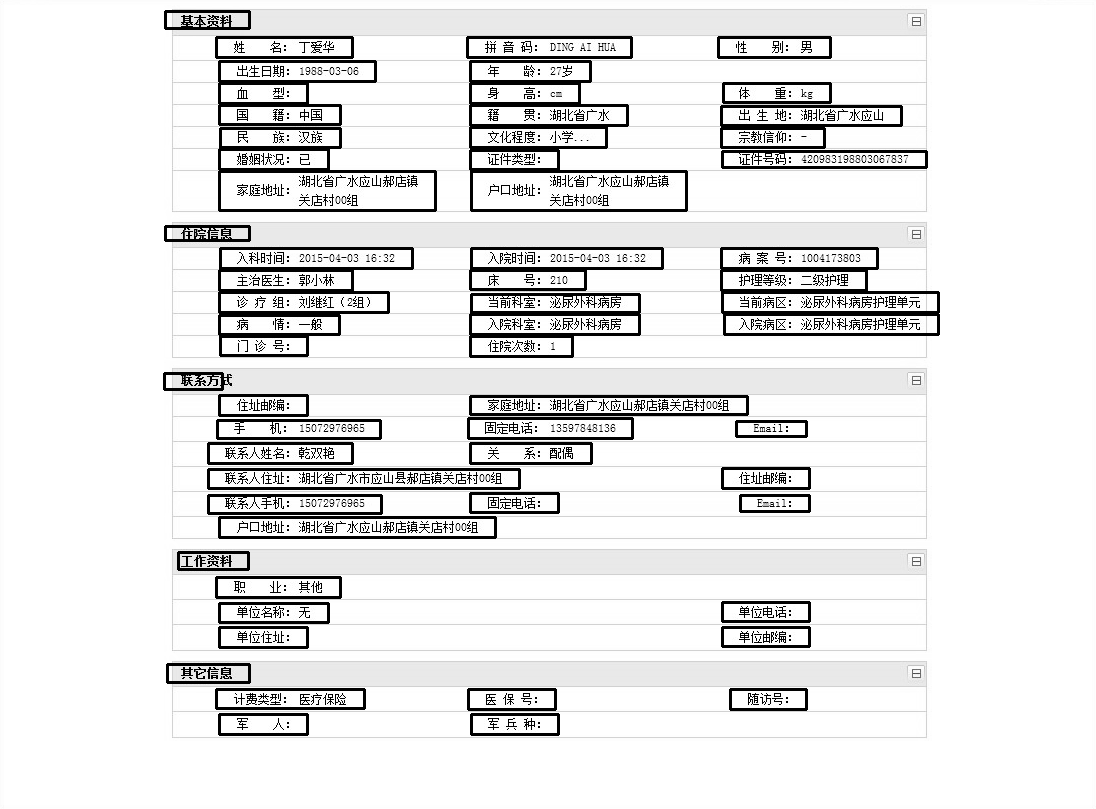
\includegraphics[width=\textwidth]{bingli1-contours}
  \end{minipage}
  }
  \caption{图片连通域分析}
  \label{pic:connected-component-analysis}
\end{figure}
连通域分析(Connected Component Analysis),是图像处理中一种常见的图片分割方法,顾名思义,它的主要作用是找到一张图片中(一般为二值图)连通的若干个子区域,并将它们从原图中划分出来,连通域分析方法在图像处理中有着广泛的应用,如人脸识别\citep{kuchi2002human},场景文字检测(Scene Text Detection)\citep{koo2013scene},网络中的社群发现(Community Detection)\citep{duch2005community}等等。另外,也有许多工作致力于快速地进行连通域分析,如优化两遍扫描法\citep{wu2009optimizing},线性时间连通域分析\citep{suzuki2003linear},并行化连通域分析\citep{han1990efficient}等等。

最常见的连通域分析方法有两遍扫描法(Two-Pass)和种子填充法(Seed Filling),两遍扫描法通过扫描两遍图像,获得全图的连通域信息并标注出来,而种子填充法则是先选取一个像素点作为种子(初始连通域),每次迭代都将与连通域相邻的像素纳入,知道找到所有属于同一连通域的像素集合,构成最终的连通域,然后重新选取种子确定下一个连通域,直到所有的连通域被找到,算法终止。在OpenCV中也内置了连通域分析函数。

我们注意到,在病历图片中,虽然字段间有一定的间隔,但字与字之间,甚至是字的内部,很多都是不连通的,如果我们直接对\autoref{pic:bingli1_contours_origin}进行连通域划分,效果会很差,因此,需要对原图片进行与前一小节类似的灰度化、二值化、腐蚀等处理,将字内部、字与字之间都连接起来,同时保持字段的分隔,\autoref{pic:bingli1_contours_origin}经过这一系列转换,我们得到如\autoref{pic:bingli1_contours_eroded}所示的二值化腐蚀图像,然后对它进行连通域分析,再将找到的连通域位置映射到原图,就得到\autoref{pic:bingli1_contours},我们看到,各个字段被矩形框框住,同时字段与字段之间很好的分隔开了,字段提取工作完成。

至此,我们完成了版面分析的全部工作。

\section{预处理模块}     % 1000字
虽然原始的病历图片并不算模糊,但是由于每个字相对来说很小,导致当我们将截取出来的字段放大来看时,每个字的笔画很模糊,有不少噪声,并且像素化明显(见\autoref{pic:image-before-processing},这是从病历图片中截取出来的一个字段),这样的文字对于文字识别来说是很困难的,因此我们需要一个预处理模块,来对文字进行放大,加粗线条,去除噪声,降低识别难度。
首先要做的就是文字的放大,在放大的过程中,为了保持文字的连贯,避免由于文字笔画太细出现中断的情况,我们需要用到插值(interpolation)算法。插值算法在图像处理领域有着广泛的运用\citep{thevenaz2000image},简单来说它是一种根据已有像素点的值来填充新像素点的方法,常用的插值方法有以下几种:
\begin{itemize}
	\item 最近邻插值,这是一种最简单的插值算法,新像素点的值由离它最近的像素点确定,即与最近的像素点的值保持一致,显然这样的话,图片会有比较明显的锯齿效应。
	\item 线性插值,是指以线性函数为插值函数的插值方法,对于最简单的一维情况,它的数学表达式可写为
		\begin{equation}
			P(x) = f_0\frac{x-x_1}{x_0-x_1}+f_1\frac{x-x_0}{x_1-x_0}
		\end{equation}
		其中,$x_0$、$x_1$分别为已知的两个像素点的坐标,$f_0$、$f_1$为它们对应的像素值,那么新像素点$x$的像素值为$P(x)$。
	\item 双线性插值,它可以被看做是线性插值的一个拓展,核心思想是在两个方向上各进行一次线性插值,叠加结果得到新像素点的像素值。
\end{itemize}
除此之外,还有双三次插值、分形插值(Fractal Interpolation)\citep{barnsley1986fractal}、边缘定向插值(Edge-directed Interpolation)\citep{li2001new}等,这里就不再一一介绍。
OpenCV中进行图片放缩的时候,支持指定自带的几种插值方法,函数原型是:
\begin{Code}
void resize(InputArray src, OutputArray dst, Size dsize, double fx=0, double fy=0, int interpolation=INTER_LINEAR )
\end{Code}
其中最后一个参数,用来指定插值方法,支持最近邻插值、双线性插值、双三次插值等。

文字经过二值化、放缩等步骤以后,最后转换成了\autoref{pic:image-after-processing},可以看到,相比于原图,图片更加纯净,去除了大量的早点,同时文字线条也更加饱满清晰,更加便于文字识别系统的识别,后续的实验也证明这大大提高了文字识别精度。至此,图片的预处理阶段完成。
\begin{figure}[htbp]
  \centering
  \subfloat[]{
  \label{pic:image-before-processing}
  \begin{minipage}[t]{0.45\textwidth}
    \centering
    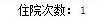
\includegraphics[width=\textwidth]{text-origin}
  \end{minipage}
  }
	\hfill
  \subfloat[]{
  \label{pic:image-after-processing}
  \begin{minipage}[t]{0.45\textwidth}
    \centering
    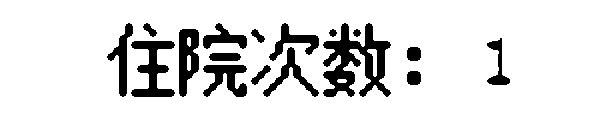
\includegraphics[width=\textwidth]{text-resized}
  \end{minipage}
  }
  \caption{文字的预处理}
  \label{pic:pre-processing}
\end{figure}

\section{OCR模块}     % 6000字
在前面的章节中,我们已经简要介绍了开源OCR引擎Tesseract的发展历史和基本现状,作为整个系统的核心模块,我们有必要对Tesseract有更加详细的了解,接下来,我们将从架构、实现细节方面来展开介绍。这部分内容主要参考自Tesseract的开发者Ray Smith的两篇文章\autoref{smith2007Tesseract,smith2013history}以及部分Tesseract的源码\footnote{Tesseract源码可见:https://github.com/tesseract-ocr/tesseract}。

\subsection{整体流程}
首先要说明的是,由于惠普公司当时在开发这套系统的时候,使用的是公司内部固定的版式,因此,从一开始Tesseract就不需要自己的版面分析系统,因此,Tesseract默认假设输入的图片数据是已经二值化的只包含若干个文本区域的图片数据。整个处理流程是比较传统的逐步管道模式(step-by-step pipeline)。

第一步是进行连通域分析,同时将识别出来的连通域轮廓保存下来,这在当时是一个计算消耗比较大的设计,不过也赋予了Tesseract一个特别的优势:通过检查嵌套的轮廓,以及子轮廓的数目,此时,文字的全部信息都被存到文字的轮廓中,已经剥离了文字的颜色信息,因此它能很容易的进行反转文字(inverse text)的识别,即“黑底白字”的识别。Tesseract被认为是首个具有比较强的翻转文字识别能力的OCR引擎。这些嵌套的轮廓聚合在一起,构成若干个文字块(Blobs)。

第二步是将这些文字块组成一行行文字,它们会根据不同的字符间距(character spacing)被划分为一个个单词。定宽(fixed pitch)的文字,会根据字符单元格(character cells)被直接划分切分成词,而不定宽(proportional)的文字则会根据绝对间距(definite spaces)和模糊间距(fuzzy spaces)来切分成词。

第三步就是文字识别。它是一个两遍(two-pass)识别过程,在第一遍时,识别系统会尝试着轮流识别每个单词。每当识别一个有可信度的单词时,这个单词就会被加入到一个自适应分类器(adaptive classifier)中,作为训练数据。这样这个自适应分类器就能在识别接下来的文字时有更高的精度。如果只过一遍网络,那么自适应分类器学到的新知识就无法应用到当前的文本中,因此,需要过第二遍识别,这一次识别的重点是第一遍中没有能够很好识别的那些文字。

最后一步处理模糊间距,检查其他可能的字体高度划分方法。

\subsection{重要细节}
上一小节,我们粗略地介绍了Tesseract的整体识别流程,帮助我们宏观地了解Tesseract的架构,接下来,我们会总结一些影响到Tesseract性能的重要细节。

\subsubsection*{缺乏版面分析能力}
就像这一节刚开始提到的那样,由于Tesseract最开始由惠普公司开发的时候,只针对惠普公司内部的特定版式,所以,它在设计之初就没有任何版面分析的模块(这也是为什么在整体流程中没有版面分析这一步),因此,Tesseract只能作为一个识别确定文本区域的文字识别模块,它的输出也只局限于文本,并没有关于版式的信息。在处理特定任务时,我们往往需要根据问题特点,自己设计实现版面分析功能,这也就是为什么很多类似于Tesseract这样的文字识别引擎不能直接用于复杂的文字识别任务。

\subsubsection*{多语言支持}
最初的Tesseract只支持英文的识别,到了Tesseract 2.0版本,加入了Unicode(UTF-8)的支持,此时支持的语言达到6种,而到了Tesseract 3.0版本,又增加了多种新语言支持,这其中就包括中文、日语、韩语。如今,它支持的语言已经将近90种,并且支持同时在一张图中识别多种语言。这些语言各不相同,每种语言都有数千种不同的形状,如果Tesseract要同时支持如此多种语言的话,字符匹配的难度无疑会大大增加,并且这种大而全的文字识别器其实并不实用,大多数情况下,需要识别的文字可能只是其中特定的一到两种,其他语言的引入反而是极大的干扰。那么Tesseract是如何做到多语言支持的同时又保证实用性呢?答案是它支持用户自定义训练集,也就是说,用户可以根据需求只将需要识别的语言加入到训练集中,让识别精度得到了有效保障。

\subsubsection*{异常字符确定}
在以中文字符为主的文本块中,偶尔会出现一些英文字符,数字,标点符号等,怎么确定哪些符号是非中文字符(或异常字符)呢?这里有一个很重要的先验知识,那就是这些异常字符一般与正常的中文字符在高度上是不一致的,如\autoref{pic:image-after-processing}中,“住院次数”在字符高度上明显比数字“1”要高,那么,当我们大体确定了整行或整篇文字的平均高度以后,那些低于平均高度的字符,就可以高可信地认为是异常字符(即英文、数字、标点等),这样我们相当于对数据做了一次划分(中文与非中文),减少了各自类型字符识别的可能情况,从而提高了识别精度(尤其是对异常字符)。

\subsubsection*{不等宽单词的划分}
不等宽单词的划分是识别中的一个难点,如\autoref{pic:difficult-word-spacing}中所示的单词“of”和“financial”,如果我们用两个边界框(bounding box)将它们框起来的话,会发现这两个单词之间并没有任何横向间隔(horizontal gap),意即计算机系统是无法根据边界框来将这两个单词划分出来的,但是人却能很明显地将它们区分开来,为什么呢?一个比较有说服力的解释是我们是从两个两个单词的中线部分能明显看到间隔。Tesseract也是利用了这个知识,在处理不等宽单词的划分时,它考量的是单词在基线(baseline)与中线(mean line)之间的某个区域内的间隔,这样就能将它们很明确的划分开来。
\begin{figure}
	\centering
	
\includegraphics[width=0.5\textwidth]{difficult-word-spacing}
	\caption{不等宽单词的划分}
	\label{pic:difficult-word-spacing}
\end{figure}

\subsubsection*{分类器候选词}
文字识别分类器在识别过程中,会给出某个待识别单词的一系列可能的候选词,以及每个候选词的置信度得分(confidence scores),之后再结合字典、前后文信息等,得到综合得分,然后选取得分最高的单词作为最后的识别结果。这个置信度得分会在切分粘连字符时用到。

\subsubsection*{粘连字符的切分}
有时候由于预处理是文字的放缩失当,会导致部分字符粘连在一起,如\autoref{pic:chopping-joint-characters}中所示单词“arm”就被粘连在一起,这样势必导致识别置信度较低,此时,Tesseract会尝试对粘连字符(置信度得分低的字块)进行切分,切分的候选点是所有轮廓多边形的凹点(concave vertices),即\autoref{pic:chopping-joint-characters}中小三角形标注的点,Tesseract会逐一按照各个凹点进行切分,重新识别,只保留置信度较高的切分方式,这样,就能正确地将三个字母正确切分出来。
\begin{figure}
	\centering
	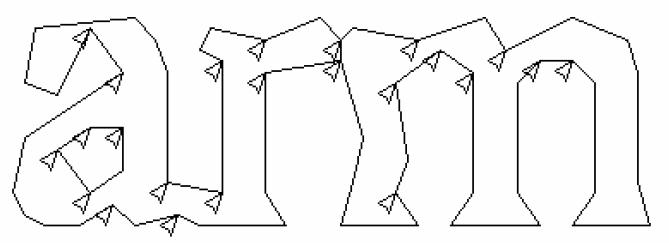
\includegraphics[width=0.5\textwidth]{chopping-joint-characters}
	\caption{粘连字符的切分}
	\label{pic:chopping-joint-characters}
\end{figure}

\subsubsection*{不同划分方法的比较}
对于同一段文本块,它即可能被划分为$A$、$B$两个单词,也有可能被划分为$C$、$D$、$E$三个单词,这时如何比较两种划分的优劣呢?如果简单的将两边每个单词的置信度相加比较肯定是不当的,因为第二种划分有3个单词,置信度相加以后的和很可能会比只有两个单词的置信度之和要大;那么将置信度之和除以单词数目之后再比较呢?这种均分置信度也有问题,因为各个单词的长度并不相等,各自在整个文本块中所占的“比重”并不一样,直接平均也不可取。因此,最终采用的计算方案如\autoref{eq:confidence-comparison}所示,由于同一段文本块的总长度$len$一定,每个单词的置信权重取决于它在整个文本块中的“比重”。
\begin{equation} \label{eq:confidence-comparison}
	\begin{split}
		&Conf(AB) = Conf(A)\frac{Len(A)}{len} + Conf(B)\frac{Len(B)}{len} \\
		&where \quad len=Len(A) + Len(B)
	\end{split}
\end{equation}

\subsubsection*{自适应分类器}
在Tesseract中,有两个分类器:静态分类器(static classifier)和自适应分类器(adaptive classifier)。由于静态分类器涉及到多种字体,通用性比较强,但是其区分相近字符、字符与非字符的能力被削弱。此时,由于每页文档内的字符的个数有限,利用静态分类器的结果可以训练出对字体更敏感的自适应分类器,可以提高分类能力。%这几句摘自http://blog.csdn.net/viewcode/article/details/7790065
Tesseract在识别时会做两遍识别,第一遍时,识别系统会尝试着轮流识别每个单词。每当识别一个有可信度的单词时,这个单词就会被加入到一个自适应分类器(adaptive classifier)中,作为训练数据。这样这个自适应分类器就能在识别接下来的文字时有更高的精度。如果只过一遍网络,那么自适应分类器学到的新知识就无法应用到当前的文本中,因此,需要过第二遍识别,这一次识别的重点是第一遍中没有能够很好识别的那些文字。%这几句与“整体流程”小节一样。
因此,自适应分类器让Tesseract具有了即时(on-the-fly)的学习能力。

\subsubsection*{分类器模型}
Tesseract中采用的分类器模型是k近邻(k-Nearest Neighbour,KNN),采用的距离度量是在特征空间里的欧几里得距离,k近邻是机器学习中比较成熟的分类模型,它的核心思路是:如果一个样本在特征空间里面k个最相似的样本中的大多数属于某一个类别,那么该样本也属于这个类别。k近邻虽然实现简单,但是它有 一个很大的缺点就是计算量比较大,因为每个样本需要与其他所有的样本进行距离计算,当特征空间维数大或者训练数据容量大时,无疑是非常耗时的。这也是Tesseract在识别速度上不如市面上很多商业化OCR软件的原因之一。
另外,Tesseract为了支持阿拉伯语专门实现了一个卷积神经网络(Convolutional neural networks,CNN)分类器,在阿拉伯语上表现很好,但在欧洲语言上,性能和效果都不行。%这一句摘自http://zhuanlan.zhihu.com/p/20231514

\subsection{字符库训练}
Tesseract官方提供了一个中文字符库\footnote{官方提供的多种语言字符库下载:https://github.com/tesseract-ocr/tessdata},用来对中文进行识别,这个字符库中包含了印刷体中文里的很多种字体,是一个大而全的字符库,

\subsection{添加用户字典}

\subsection{其他细节}
值得一提的是,在Windows平台,Tesseract识别的文本在显示时会出现大量的乱码问题,这是因为Windows平台默认的文本代码存储方式是UTF8-WithBOM,而Tesseract引擎识别后产出的文本是以标准UTF8格式的,直接输出势必会产生乱码。因此(在Windows平台)我们需要对文本进行转码,具体的转码步骤是先将UTF8转换成Unicode格式,然后将Unicode转换成Ansi字符标准格式,这两个转换函数如下所示:
\begin{lstlisting}[numbers=none]
wchar_t * Utf_8ToUnicode(char* szU8)
{
	int wcsLen = ::MultiByteToWideChar(CP_UTF8, NULL, szU8, strlen(szU8), NULL, 0);
	wchar_t* wszString = new wchar_t[wcsLen + 1];
	::MultiByteToWideChar(CP_UTF8, NULL, szU8, strlen(szU8), wszString, wcsLen);
	wszString[wcsLen] = '\0';
	return wszString;
}

char* UnicodeToAnsi( const wchar_t* szStr )
{
	int nLen = WideCharToMultiByte( CP_ACP, 0, szStr, -1, NULL, 0, NULL, NULL );
	if (nLen == 0)
		return NULL;
	char* pResult = new char[nLen];
	WideCharToMultiByte( CP_ACP, 0, szStr, -1, pResult, nLen, NULL, NULL );
	return pResult;
}
\end{lstlisting}

\section{字段解析模块}  %2000字
当含有文本的图片数据经过OCR模块以后,会被转换为文本,这些文本需要进行一定的加工,才能得到我们想要的各字段数据。总体来说,原始的文本需要经过数据清洗、字段匹配、目标文本提取等步骤。我们也可以认为这是数据的“后处理”过程。

\subsection{数据清洗}
数据清洗主要有两大功能,一是对文本的冗余信息进行剔除,二是对文本进行简单的矫正。这两部分实现难度不大,却对之后的字段匹配过程有着很大的帮助。

识别的文本中可能包含冗余信息,如因为图片噪声而产生的冗余符号,或者是图片中没用实际意义的标题栏等等,剔除这些冗余信息的方法是维护一个“异常字符列表”,将一些不常见的字符加入列表中,如果识别的文本中包含这些字符,就将其剔除。

另外,由于OCR模块的单词切分不一定准确,对于有些词的切分可能会错误切分,这种错误切分往往是重复且稳定复现的,比如“日期”两个字,OCR可能会“稳定地”将其错误识别为“日月其”,这在日常语境下是极少会出现的。因此,我们也可以维护一个“错误切分列表”,将这些稳定复现的错误切分词进行矫正。

\subsection{字段匹配}
某段文本属于哪一个字段呢?这就需要对文本的具体内容进行理解划分了,字段匹配大体上分为StartsWith匹配和Include匹配两种。
\subsubsection*{StartsWith匹配}
所谓StartsWith匹配,是指那些以字段名开头的文本,比如“姓名:某某某”,我们可以直接通过开头的文字来判断字段,并去除字段名得到字段的实际内容。因此,我们可以维护一个在文本最开头出现的字段名“StartsWith”列表,系统可以通过查询列表来进行字段匹配。
\subsubsection*{Includes匹配}
有些文本则并不是以字段名开头,比如\autoref{pic:IncludesWith-example}中显示的字段,由于文字高度不同,OCR引擎不会最先识别“家庭住址:”,导致这个字段名会隐藏在文本的中段,因此,我们需要维护一个在文本中段出现的字段名“IncludesWith”列表,同时运用一些子字符串匹配的高效算法进行字段匹配,去除字段名得到字段的实际内容。在本系统中用到的子字符串匹配算法为AC多模匹配算法(Aho-Corasick algorithm)\citep{aho1975efficient},它是计算机科学中常见的一种字符串匹配算法,算法时间复杂度能达到$O(n)$,为本系统的子字符串匹配提供了效率保障。
\begin{figure}
	\centering
	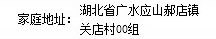
\includegraphics[width=0.5\textwidth]{IncludesWith-example}
	\caption{不以字段名为开头的字段举例}
	\label{pic:IncludesWith-example}
\end{figure}


\section{数据存储模块} %500字
当字段解析完成后,最后一步就是存储,根据\autoref{ssub:requirements-dataWriter}中的需求分析,存储的数据格式应该是可用excel打开,便于展示的,常见的excel文件读写方式有以下几种:
\begin{itemize}
	\item OLE(Object Linking and Embedding)方式。它的原理是启动一个EXCEL的进程来读写excel文件,它的优点是功能强大,能满足各种excel操作,缺点是读写速度慢,并且这种方式是不可移植的,且必须已经安装EXCEL。
	\item LibXL方式。LibXL是一个收费的EXCEL库\footnote{LibXL网址:http://www.libxl.com/},优点是可以不依赖EXCEL来读取xls文件,操作简单,缺点当然是需要收费。
	\item ODBC(Open Database Connectivity)方式。ODBC是微软提出的数据库访问接口标准,采用这种方式读取excel可以做丰富的数据库管理操作,缺点是读写速度慢,另外需要安装excel驱动程序。
\end{itemize}
我们需要存储的数据只是需要用excel作为简单的展示平台,本身并不需要其他的excel操作,因此以上几种方式事实上都是功能过剩,存储效率比较低,而且需要已经安装EXCEL,无法跨平台。本系统最后采用的解决方案是将病历数据存储为csv格式的文本文档,CSV(Comma-Separated Values),是一种文件存储格式,以纯文本形式来存储表格数据,它的这个特性带来了如下几个优点:
\begin{itemize}
	\item 读写速度快,因为它是一种纯文本格式,所以可以很快地进行文本读写操作;
	\item 可以直接被EXCEL识别为正确的表格文件,让数据拥有更好的展示效果;
	\item 不依赖EXCEL程序本身,这样它就能做到跨平台。
\end{itemize}
因此,csv格式存储已经满足了本系统的所有需求,是综合考虑以后最优的解决方案。

\section{小结}
